%Chapter 4
\chapter{Results and validation}
\thispagestyle{empty}
\vspace{38em}
\hrulefill
\\
\enquote*{\textit{Quote.}} - Somebody\\
\newpage
\section{Introduction}
This section will discuss the results of the implementing the simulation methodology on various case case study. Further, the result of various simulated scenarios will be discussed. Finally validation of the the simulated scenarios using actual measurable tests will be discussed.
\section{Case study A}
{\color{blue}(Beatrix 123)}
\subsection{System investigation}
Case study A represents a group of three gold mining shafts and a gold processing plant in the Free state that share a compressed air network. Prior to this study, efforts were made to optimise the system through \gls{dsm} energy projects. An investigation into the system was performed to identify potential energy and operation improvements strategies that are still available.
\par 
An air distribution layout was developed for the system, the simplified diagram is shown in Figure \ref{fig: Beatrix Air layout}.From this along with information from the mine personal and system data, an understanding of the operation philosophy was obtained. 
\par 
\begin{figure}[h!]
	\centering
	\fbox{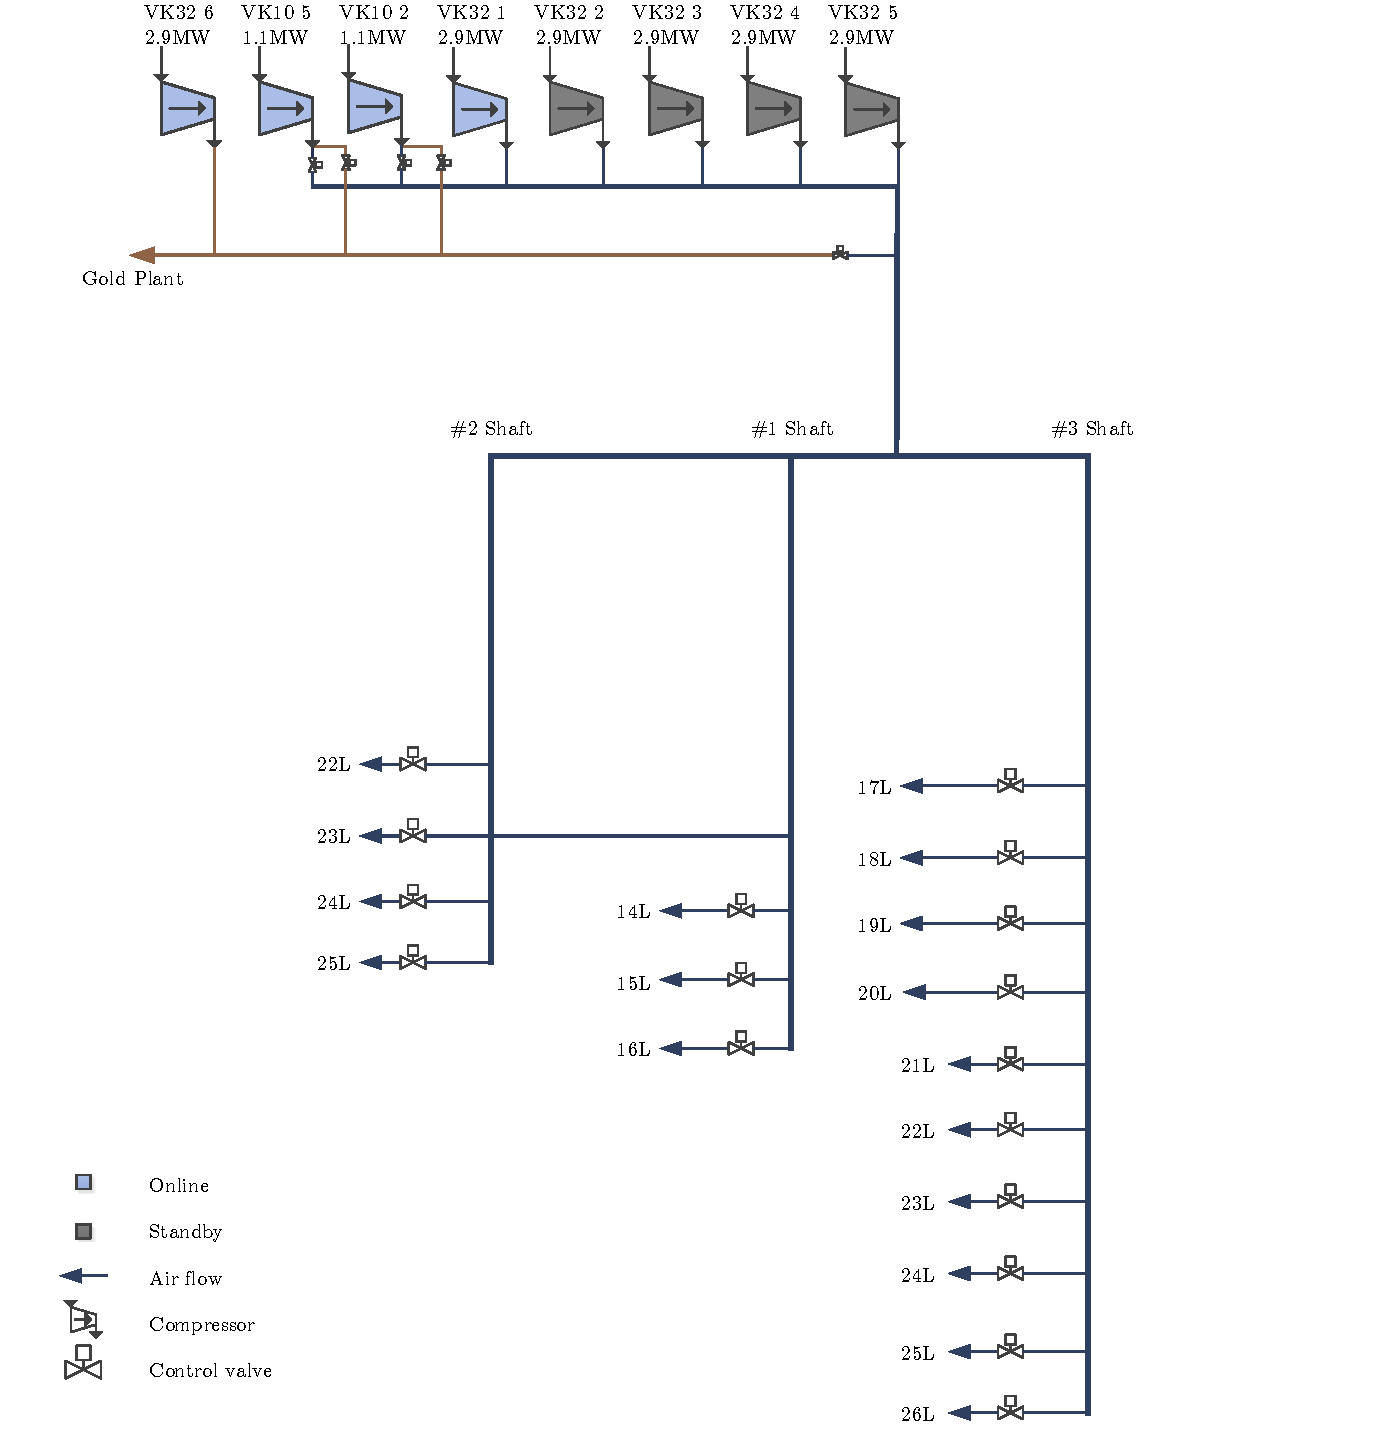
\includegraphics[trim =0cm 0.6cm 0cm 0.6cm,width=\textwidth]{Graphs/4/BeatLayout1/BeatLayout1.pdf}}
	\caption{Simplified air distribution of the air network.}
	\label{fig: Beatrix Air layout}
\end{figure}


Seven compresses are available in the system. Five large compressors (VK32s) rated at 4 $MW$ each and two smaller compressors (VK10) with a power rating of 2.1 $MW$ each. The system is typically supplied using combination of 2 VK32 compressors and 2 VK 10 compressors. The rest of the compressors are used as standby. Compressors are shut off or switched on  to match the demand in the system.  
\par
Air is supplied to the sections in three mining shafts as well as a gold processing plant. The gold plant requires constant high pressure throughout the day. It is possible to control the supply pressure of the gold plant independently from the rest of the network. However the mine prefers to operate the network with a constant pressure setpoint. A more detailed air distribution layout including location of flow meters is shown in "Appendix A". 
\subsection{Model development}
Using the data and knowledge gathered from  the investigation, a model was developed using the methodology discussed in Chapter 3.
\subsubsection{Verification of model}

\begin{figure}[h]
	\centering
	\fbox{% GNUPLOT: LaTeX picture with Postscript
\begingroup
  \makeatletter
  \providecommand\color[2][]{%
    \GenericError{(gnuplot) \space\space\space\@spaces}{%
      Package color not loaded in conjunction with
      terminal option `colourtext'%
    }{See the gnuplot documentation for explanation.%
    }{Either use 'blacktext' in gnuplot or load the package
      color.sty in LaTeX.}%
    \renewcommand\color[2][]{}%
  }%
  \providecommand\includegraphics[2][]{%
    \GenericError{(gnuplot) \space\space\space\@spaces}{%
      Package graphicx or graphics not loaded%
    }{See the gnuplot documentation for explanation.%
    }{The gnuplot epslatex terminal needs graphicx.sty or graphics.sty.}%
    \renewcommand\includegraphics[2][]{}%
  }%
  \providecommand\rotatebox[2]{#2}%
  \@ifundefined{ifGPcolor}{%
    \newif\ifGPcolor
    \GPcolortrue
  }{}%
  \@ifundefined{ifGPblacktext}{%
    \newif\ifGPblacktext
    \GPblacktextfalse
  }{}%
  % define a \g@addto@macro without @ in the name:
  \let\gplgaddtomacro\g@addto@macro
  % define empty templates for all commands taking text:
  \gdef\gplbacktext{}%
  \gdef\gplfronttext{}%
  \makeatother
  \ifGPblacktext
    % no textcolor at all
    \def\colorrgb#1{}%
    \def\colorgray#1{}%
  \else
    % gray or color?
    \ifGPcolor
      \def\colorrgb#1{\color[rgb]{#1}}%
      \def\colorgray#1{\color[gray]{#1}}%
      \expandafter\def\csname LTw\endcsname{\color{white}}%
      \expandafter\def\csname LTb\endcsname{\color{black}}%
      \expandafter\def\csname LTa\endcsname{\color{black}}%
      \expandafter\def\csname LT0\endcsname{\color[rgb]{1,0,0}}%
      \expandafter\def\csname LT1\endcsname{\color[rgb]{0,1,0}}%
      \expandafter\def\csname LT2\endcsname{\color[rgb]{0,0,1}}%
      \expandafter\def\csname LT3\endcsname{\color[rgb]{1,0,1}}%
      \expandafter\def\csname LT4\endcsname{\color[rgb]{0,1,1}}%
      \expandafter\def\csname LT5\endcsname{\color[rgb]{1,1,0}}%
      \expandafter\def\csname LT6\endcsname{\color[rgb]{0,0,0}}%
      \expandafter\def\csname LT7\endcsname{\color[rgb]{1,0.3,0}}%
      \expandafter\def\csname LT8\endcsname{\color[rgb]{0.5,0.5,0.5}}%
    \else
      % gray
      \def\colorrgb#1{\color{black}}%
      \def\colorgray#1{\color[gray]{#1}}%
      \expandafter\def\csname LTw\endcsname{\color{white}}%
      \expandafter\def\csname LTb\endcsname{\color{black}}%
      \expandafter\def\csname LTa\endcsname{\color{black}}%
      \expandafter\def\csname LT0\endcsname{\color{black}}%
      \expandafter\def\csname LT1\endcsname{\color{black}}%
      \expandafter\def\csname LT2\endcsname{\color{black}}%
      \expandafter\def\csname LT3\endcsname{\color{black}}%
      \expandafter\def\csname LT4\endcsname{\color{black}}%
      \expandafter\def\csname LT5\endcsname{\color{black}}%
      \expandafter\def\csname LT6\endcsname{\color{black}}%
      \expandafter\def\csname LT7\endcsname{\color{black}}%
      \expandafter\def\csname LT8\endcsname{\color{black}}%
    \fi
  \fi
    \setlength{\unitlength}{0.0500bp}%
    \ifx\gptboxheight\undefined%
      \newlength{\gptboxheight}%
      \newlength{\gptboxwidth}%
      \newsavebox{\gptboxtext}%
    \fi%
    \setlength{\fboxrule}{0.5pt}%
    \setlength{\fboxsep}{1pt}%
\begin{picture}(9360.00,4032.00)%
    \gplgaddtomacro\gplbacktext{%
      \colorrgb{0.00,0.00,0.00}%
      \put(550,924){\makebox(0,0)[r]{\strut{}$0$}}%
      \colorrgb{0.00,0.00,0.00}%
      \put(550,1279){\makebox(0,0)[r]{\strut{}$1$}}%
      \colorrgb{0.00,0.00,0.00}%
      \put(550,1635){\makebox(0,0)[r]{\strut{}$2$}}%
      \colorrgb{0.00,0.00,0.00}%
      \put(550,1990){\makebox(0,0)[r]{\strut{}$3$}}%
      \colorrgb{0.00,0.00,0.00}%
      \put(550,2346){\makebox(0,0)[r]{\strut{}$4$}}%
      \colorrgb{0.00,0.00,0.00}%
      \put(550,2701){\makebox(0,0)[r]{\strut{}$5$}}%
      \colorrgb{0.00,0.00,0.00}%
      \put(550,3056){\makebox(0,0)[r]{\strut{}$6$}}%
      \colorrgb{0.00,0.00,0.00}%
      \put(550,3412){\makebox(0,0)[r]{\strut{}$7$}}%
      \colorrgb{0.00,0.00,0.00}%
      \put(550,3767){\makebox(0,0)[r]{\strut{}$8$}}%
      \colorrgb{0.00,0.00,0.00}%
      \put(682,704){\makebox(0,0){\strut{}00:00}}%
      \colorrgb{0.00,0.00,0.00}%
      \put(1937,704){\makebox(0,0){\strut{}04:00}}%
      \colorrgb{0.00,0.00,0.00}%
      \put(3193,704){\makebox(0,0){\strut{}08:00}}%
      \colorrgb{0.00,0.00,0.00}%
      \put(4448,704){\makebox(0,0){\strut{}12:00}}%
      \colorrgb{0.00,0.00,0.00}%
      \put(5703,704){\makebox(0,0){\strut{}16:00}}%
      \colorrgb{0.00,0.00,0.00}%
      \put(6959,704){\makebox(0,0){\strut{}20:00}}%
      \colorrgb{0.00,0.00,0.00}%
      \put(8214,704){\makebox(0,0){\strut{}00:00}}%
      \colorrgb{0.00,0.00,0.00}%
      \put(8346,924){\makebox(0,0)[l]{\strut{}$0$}}%
      \colorrgb{0.00,0.00,0.00}%
      \put(8346,2061){\makebox(0,0)[l]{\strut{}$10$}}%
      \colorrgb{0.00,0.00,0.00}%
      \put(8346,3198){\makebox(0,0)[l]{\strut{}$20$}}%
    }%
    \gplgaddtomacro\gplfronttext{%
      \csname LTb\endcsname%
      \put(176,2345){\rotatebox{-270}{\makebox(0,0){\strut{}Power $(MW)$}}}%
      \put(8851,2345){\rotatebox{-270}{\makebox(0,0){\strut{}$\%$ $error$}}}%
      \put(4448,374){\makebox(0,0){\strut{}Time of use}}%
      \csname LTb\endcsname%
      \put(2175,173){\makebox(0,0)[r]{\strut{}Baseline power}}%
      \csname LTb\endcsname%
      \put(5010,173){\makebox(0,0)[r]{\strut{}Simulated power}}%
      \csname LTb\endcsname%
      \put(7700,173){\makebox(0,0)[r]{\strut{}Rel. Error}}%
    }%
    \gplbacktext
    \put(0,0){\fbox{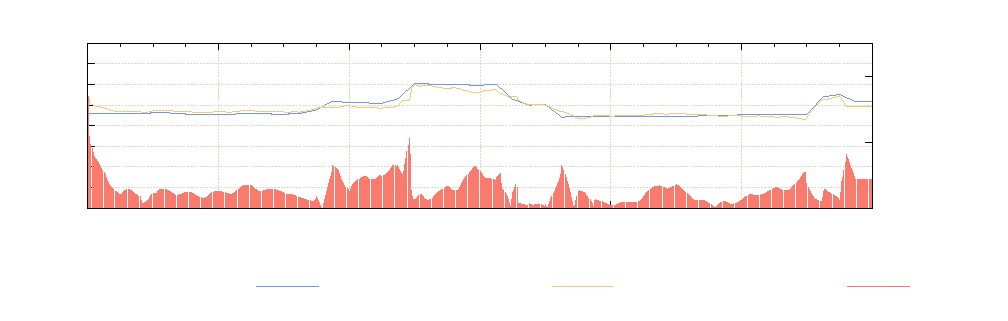
\includegraphics[trim=0 0 0.1cm 0, clip]{Graphs/4/BeetVerify/Power/Power}}}%
    \gplfronttext
  \end{picture}%
\endgroup
}
	\caption{The simulated power compared to the actual measured power}
	\label{fig: Verification Power Beatrix}
\end{figure}

\begin{figure}[h]
	\centering
	\fbox{% GNUPLOT: LaTeX picture with Postscript
\begingroup
  \makeatletter
  \providecommand\color[2][]{%
    \GenericError{(gnuplot) \space\space\space\@spaces}{%
      Package color not loaded in conjunction with
      terminal option `colourtext'%
    }{See the gnuplot documentation for explanation.%
    }{Either use 'blacktext' in gnuplot or load the package
      color.sty in LaTeX.}%
    \renewcommand\color[2][]{}%
  }%
  \providecommand\includegraphics[2][]{%
    \GenericError{(gnuplot) \space\space\space\@spaces}{%
      Package graphicx or graphics not loaded%
    }{See the gnuplot documentation for explanation.%
    }{The gnuplot epslatex terminal needs graphicx.sty or graphics.sty.}%
    \renewcommand\includegraphics[2][]{}%
  }%
  \providecommand\rotatebox[2]{#2}%
  \@ifundefined{ifGPcolor}{%
    \newif\ifGPcolor
    \GPcolortrue
  }{}%
  \@ifundefined{ifGPblacktext}{%
    \newif\ifGPblacktext
    \GPblacktextfalse
  }{}%
  % define a \g@addto@macro without @ in the name:
  \let\gplgaddtomacro\g@addto@macro
  % define empty templates for all commands taking text:
  \gdef\gplbacktext{}%
  \gdef\gplfronttext{}%
  \makeatother
  \ifGPblacktext
    % no textcolor at all
    \def\colorrgb#1{}%
    \def\colorgray#1{}%
  \else
    % gray or color?
    \ifGPcolor
      \def\colorrgb#1{\color[rgb]{#1}}%
      \def\colorgray#1{\color[gray]{#1}}%
      \expandafter\def\csname LTw\endcsname{\color{white}}%
      \expandafter\def\csname LTb\endcsname{\color{black}}%
      \expandafter\def\csname LTa\endcsname{\color{black}}%
      \expandafter\def\csname LT0\endcsname{\color[rgb]{1,0,0}}%
      \expandafter\def\csname LT1\endcsname{\color[rgb]{0,1,0}}%
      \expandafter\def\csname LT2\endcsname{\color[rgb]{0,0,1}}%
      \expandafter\def\csname LT3\endcsname{\color[rgb]{1,0,1}}%
      \expandafter\def\csname LT4\endcsname{\color[rgb]{0,1,1}}%
      \expandafter\def\csname LT5\endcsname{\color[rgb]{1,1,0}}%
      \expandafter\def\csname LT6\endcsname{\color[rgb]{0,0,0}}%
      \expandafter\def\csname LT7\endcsname{\color[rgb]{1,0.3,0}}%
      \expandafter\def\csname LT8\endcsname{\color[rgb]{0.5,0.5,0.5}}%
    \else
      % gray
      \def\colorrgb#1{\color{black}}%
      \def\colorgray#1{\color[gray]{#1}}%
      \expandafter\def\csname LTw\endcsname{\color{white}}%
      \expandafter\def\csname LTb\endcsname{\color{black}}%
      \expandafter\def\csname LTa\endcsname{\color{black}}%
      \expandafter\def\csname LT0\endcsname{\color{black}}%
      \expandafter\def\csname LT1\endcsname{\color{black}}%
      \expandafter\def\csname LT2\endcsname{\color{black}}%
      \expandafter\def\csname LT3\endcsname{\color{black}}%
      \expandafter\def\csname LT4\endcsname{\color{black}}%
      \expandafter\def\csname LT5\endcsname{\color{black}}%
      \expandafter\def\csname LT6\endcsname{\color{black}}%
      \expandafter\def\csname LT7\endcsname{\color{black}}%
      \expandafter\def\csname LT8\endcsname{\color{black}}%
    \fi
  \fi
    \setlength{\unitlength}{0.0500bp}%
    \ifx\gptboxheight\undefined%
      \newlength{\gptboxheight}%
      \newlength{\gptboxwidth}%
      \newsavebox{\gptboxtext}%
    \fi%
    \setlength{\fboxrule}{0.5pt}%
    \setlength{\fboxsep}{1pt}%
\begin{picture}(9360.00,4032.00)%
    \gplgaddtomacro\gplbacktext{%
      \colorrgb{0.00,0.00,0.00}%
      \put(682,924){\makebox(0,0)[r]{\strut{}$0$}}%
      \colorrgb{0.00,0.00,0.00}%
      \put(682,1872){\makebox(0,0)[r]{\strut{}$5$}}%
      \colorrgb{0.00,0.00,0.00}%
      \put(682,2819){\makebox(0,0)[r]{\strut{}$10$}}%
      \colorrgb{0.00,0.00,0.00}%
      \put(682,3767){\makebox(0,0)[r]{\strut{}$15$}}%
      \colorrgb{0.00,0.00,0.00}%
      \put(814,704){\makebox(0,0){\strut{}00:00}}%
      \colorrgb{0.00,0.00,0.00}%
      \put(2047,704){\makebox(0,0){\strut{}04:00}}%
      \colorrgb{0.00,0.00,0.00}%
      \put(3281,704){\makebox(0,0){\strut{}08:00}}%
      \colorrgb{0.00,0.00,0.00}%
      \put(4514,704){\makebox(0,0){\strut{}12:00}}%
      \colorrgb{0.00,0.00,0.00}%
      \put(5747,704){\makebox(0,0){\strut{}16:00}}%
      \colorrgb{0.00,0.00,0.00}%
      \put(6981,704){\makebox(0,0){\strut{}20:00}}%
      \colorrgb{0.00,0.00,0.00}%
      \put(8214,704){\makebox(0,0){\strut{}00:00}}%
      \colorrgb{0.00,0.00,0.00}%
      \put(8346,924){\makebox(0,0)[l]{\strut{}$0$}}%
      \colorrgb{0.00,0.00,0.00}%
      \put(8346,2061){\makebox(0,0)[l]{\strut{}$10$}}%
      \colorrgb{0.00,0.00,0.00}%
      \put(8346,3198){\makebox(0,0)[l]{\strut{}$20$}}%
    }%
    \gplgaddtomacro\gplfronttext{%
      \csname LTb\endcsname%
      \put(176,2345){\rotatebox{-270}{\makebox(0,0){\strut{}Flow $(kg/s)$}}}%
      \put(8851,2345){\rotatebox{-270}{\makebox(0,0){\strut{}$\% error$}}}%
      \put(4514,374){\makebox(0,0){\strut{}Time of Day}}%
      \csname LTb\endcsname%
      \put(2307,173){\makebox(0,0)[r]{\strut{}Baseline flow}}%
      \csname LTb\endcsname%
      \put(5010,173){\makebox(0,0)[r]{\strut{}Simulated flow}}%
      \csname LTb\endcsname%
      \put(7713,173){\makebox(0,0)[r]{\strut{}Error}}%
    }%
    \gplbacktext
    \put(0,0){\fbox{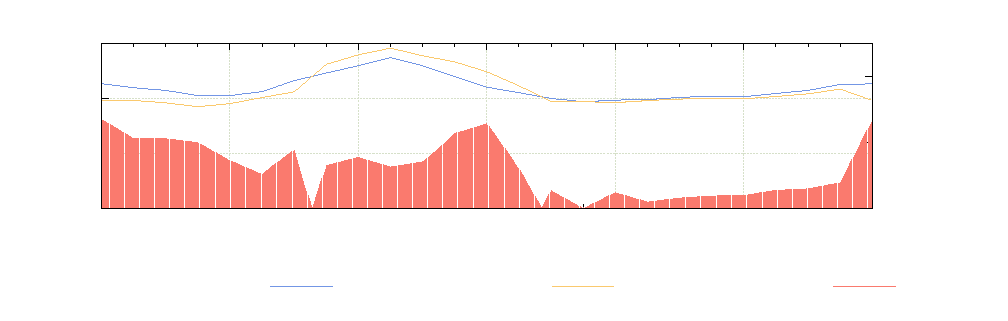
\includegraphics[trim=0 0 0.1cm 0, clip]{Graphs/4/BeetVerify/Flow/Flow}}}%
    \gplfronttext
  \end{picture}%
\endgroup
}
	\caption{The simulated flow compared to the actual measured flow}
	\label{fig: Verification Flow Beatrix}
\end{figure}

\begin{figure}[h]
	\centering
	\fbox{% GNUPLOT: LaTeX picture with Postscript
\begingroup
  \makeatletter
  \providecommand\color[2][]{%
    \GenericError{(gnuplot) \space\space\space\@spaces}{%
      Package color not loaded in conjunction with
      terminal option `colourtext'%
    }{See the gnuplot documentation for explanation.%
    }{Either use 'blacktext' in gnuplot or load the package
      color.sty in LaTeX.}%
    \renewcommand\color[2][]{}%
  }%
  \providecommand\includegraphics[2][]{%
    \GenericError{(gnuplot) \space\space\space\@spaces}{%
      Package graphicx or graphics not loaded%
    }{See the gnuplot documentation for explanation.%
    }{The gnuplot epslatex terminal needs graphicx.sty or graphics.sty.}%
    \renewcommand\includegraphics[2][]{}%
  }%
  \providecommand\rotatebox[2]{#2}%
  \@ifundefined{ifGPcolor}{%
    \newif\ifGPcolor
    \GPcolortrue
  }{}%
  \@ifundefined{ifGPblacktext}{%
    \newif\ifGPblacktext
    \GPblacktextfalse
  }{}%
  % define a \g@addto@macro without @ in the name:
  \let\gplgaddtomacro\g@addto@macro
  % define empty templates for all commands taking text:
  \gdef\gplbacktext{}%
  \gdef\gplfronttext{}%
  \makeatother
  \ifGPblacktext
    % no textcolor at all
    \def\colorrgb#1{}%
    \def\colorgray#1{}%
  \else
    % gray or color?
    \ifGPcolor
      \def\colorrgb#1{\color[rgb]{#1}}%
      \def\colorgray#1{\color[gray]{#1}}%
      \expandafter\def\csname LTw\endcsname{\color{white}}%
      \expandafter\def\csname LTb\endcsname{\color{black}}%
      \expandafter\def\csname LTa\endcsname{\color{black}}%
      \expandafter\def\csname LT0\endcsname{\color[rgb]{1,0,0}}%
      \expandafter\def\csname LT1\endcsname{\color[rgb]{0,1,0}}%
      \expandafter\def\csname LT2\endcsname{\color[rgb]{0,0,1}}%
      \expandafter\def\csname LT3\endcsname{\color[rgb]{1,0,1}}%
      \expandafter\def\csname LT4\endcsname{\color[rgb]{0,1,1}}%
      \expandafter\def\csname LT5\endcsname{\color[rgb]{1,1,0}}%
      \expandafter\def\csname LT6\endcsname{\color[rgb]{0,0,0}}%
      \expandafter\def\csname LT7\endcsname{\color[rgb]{1,0.3,0}}%
      \expandafter\def\csname LT8\endcsname{\color[rgb]{0.5,0.5,0.5}}%
    \else
      % gray
      \def\colorrgb#1{\color{black}}%
      \def\colorgray#1{\color[gray]{#1}}%
      \expandafter\def\csname LTw\endcsname{\color{white}}%
      \expandafter\def\csname LTb\endcsname{\color{black}}%
      \expandafter\def\csname LTa\endcsname{\color{black}}%
      \expandafter\def\csname LT0\endcsname{\color{black}}%
      \expandafter\def\csname LT1\endcsname{\color{black}}%
      \expandafter\def\csname LT2\endcsname{\color{black}}%
      \expandafter\def\csname LT3\endcsname{\color{black}}%
      \expandafter\def\csname LT4\endcsname{\color{black}}%
      \expandafter\def\csname LT5\endcsname{\color{black}}%
      \expandafter\def\csname LT6\endcsname{\color{black}}%
      \expandafter\def\csname LT7\endcsname{\color{black}}%
      \expandafter\def\csname LT8\endcsname{\color{black}}%
    \fi
  \fi
    \setlength{\unitlength}{0.0500bp}%
    \ifx\gptboxheight\undefined%
      \newlength{\gptboxheight}%
      \newlength{\gptboxwidth}%
      \newsavebox{\gptboxtext}%
    \fi%
    \setlength{\fboxrule}{0.5pt}%
    \setlength{\fboxsep}{1pt}%
\begin{picture}(9360.00,2772.00)%
    \gplgaddtomacro\gplbacktext{%
      \colorrgb{0.00,0.00,0.00}%
      \put(814,924){\makebox(0,0)[r]{\strut{}$300$}}%
      \colorrgb{0.00,0.00,0.00}%
      \put(814,1452){\makebox(0,0)[r]{\strut{}$350$}}%
      \colorrgb{0.00,0.00,0.00}%
      \put(814,1979){\makebox(0,0)[r]{\strut{}$400$}}%
      \colorrgb{0.00,0.00,0.00}%
      \put(814,2507){\makebox(0,0)[r]{\strut{}$450$}}%
      \colorrgb{0.00,0.00,0.00}%
      \put(946,704){\makebox(0,0){\strut{}00:00}}%
      \colorrgb{0.00,0.00,0.00}%
      \put(2157,704){\makebox(0,0){\strut{}04:00}}%
      \colorrgb{0.00,0.00,0.00}%
      \put(3369,704){\makebox(0,0){\strut{}08:00}}%
      \colorrgb{0.00,0.00,0.00}%
      \put(4580,704){\makebox(0,0){\strut{}12:00}}%
      \colorrgb{0.00,0.00,0.00}%
      \put(5791,704){\makebox(0,0){\strut{}16:00}}%
      \colorrgb{0.00,0.00,0.00}%
      \put(7003,704){\makebox(0,0){\strut{}20:00}}%
      \colorrgb{0.00,0.00,0.00}%
      \put(8214,704){\makebox(0,0){\strut{}00:00}}%
      \colorrgb{0.00,0.00,0.00}%
      \put(8346,924){\makebox(0,0)[l]{\strut{}$0$}}%
      \colorrgb{0.00,0.00,0.00}%
      \put(8346,1557){\makebox(0,0)[l]{\strut{}$10$}}%
      \colorrgb{0.00,0.00,0.00}%
      \put(8346,2190){\makebox(0,0)[l]{\strut{}$20$}}%
    }%
    \gplgaddtomacro\gplfronttext{%
      \csname LTb\endcsname%
      \put(176,1715){\rotatebox{-270}{\makebox(0,0){\strut{}Pressure $(kPa)$}}}%
      \put(8851,1715){\rotatebox{-270}{\makebox(0,0){\strut{}$\% error$}}}%
      \put(4580,374){\makebox(0,0){\strut{}Time of Day}}%
      \csname LTb\endcsname%
      \put(2241,173){\makebox(0,0)[r]{\strut{}Baseline press.}}%
      \csname LTb\endcsname%
      \put(5208,173){\makebox(0,0)[r]{\strut{}Simulated press.}}%
      \csname LTb\endcsname%
      \put(8175,173){\makebox(0,0)[r]{\strut{}Error}}%
    }%
    \gplbacktext
    \put(0,0){
\includegraphics{Graphs/4/BeetVerify/Pressure/Pressure}}%
    \gplfronttext
  \end{picture}%
\endgroup
}
	\caption{The simulated Pressure compared to the actual measured pressure}
	\label{fig: Verification Pressure Beatrix}
\end{figure}

\subsection{Scenario 1. Compressor set points}
\subsection{Scenario 2. Control valves set points}
\subsection{Validation of results}
\subsection{Summary}
\newpage
\section{Case study B }
{\color{blue}(Kusasalethu)}
	\subsection{System investigation}
	Case study B is another large South African gold mine. The mine utilises five compressors supply compressed air to various surface and underground operations. An investigation was performed to gather the data and information required to build a simulation model of the network.
	\par 
	A basic air distribution layout was obtained, as shown in Figure \ref{fig: KUS Air layout}.  The more detailed layout in !!Appendix *!!,  indicates available meters and instrumentation as well as typical airflow splits to various sections and levels of the mine.
	\par 
	
	\begin{figure}[h!]
		\centering
		\fbox{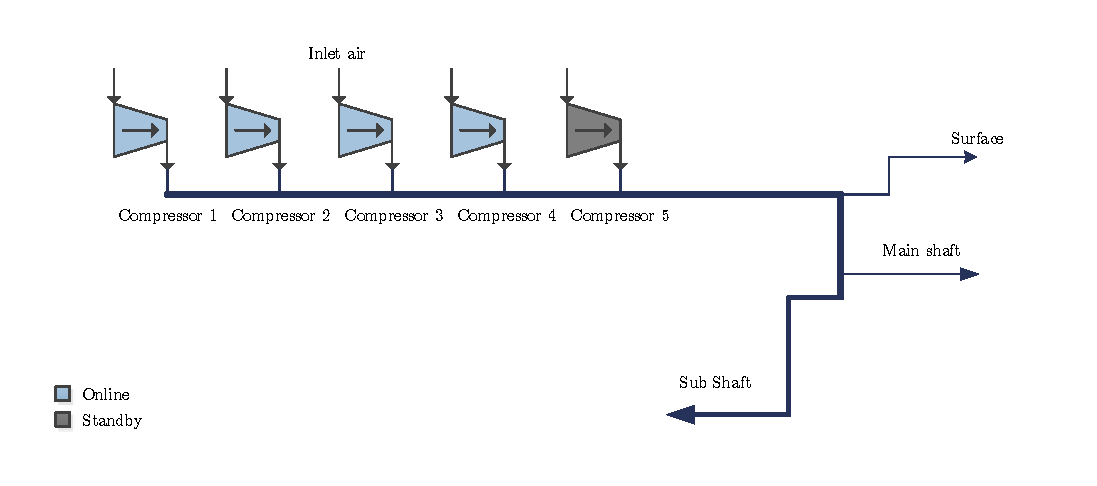
\includegraphics[trim =0cm 0.6cm 0cm 0.6cm,width=\textwidth]{Graphs/4/KUSLayout1/KUSLayout1.pdf}}
		\caption{Basic layout of the compressed air network.}
		\label{fig: KUS Air layout}
	\end{figure}
 To understand the operation of the system, schedules and setpoints as well as critical limits such as minimum and maximum pressures were obtained from various personal and from the \gls{scada}. Important data parameters such as Powers, pressures, flows, etc. for the system was gathered from the \gls{scada} and other data sources. This data will be used to develop and calibrate the simulation model
\par 
		
	An in-depth investigation was performed on the significant mining levels to map the locations of mining cross-sections, refuge bays, major leaks and other compressed air consumers on each level as well as measure the usages. An example of a resultant schematic from the underground investigation is shown in Figure \ref{fig: KUS Underground level layout}
	
	\begin{figure}[h!]
		\centering
		\fbox{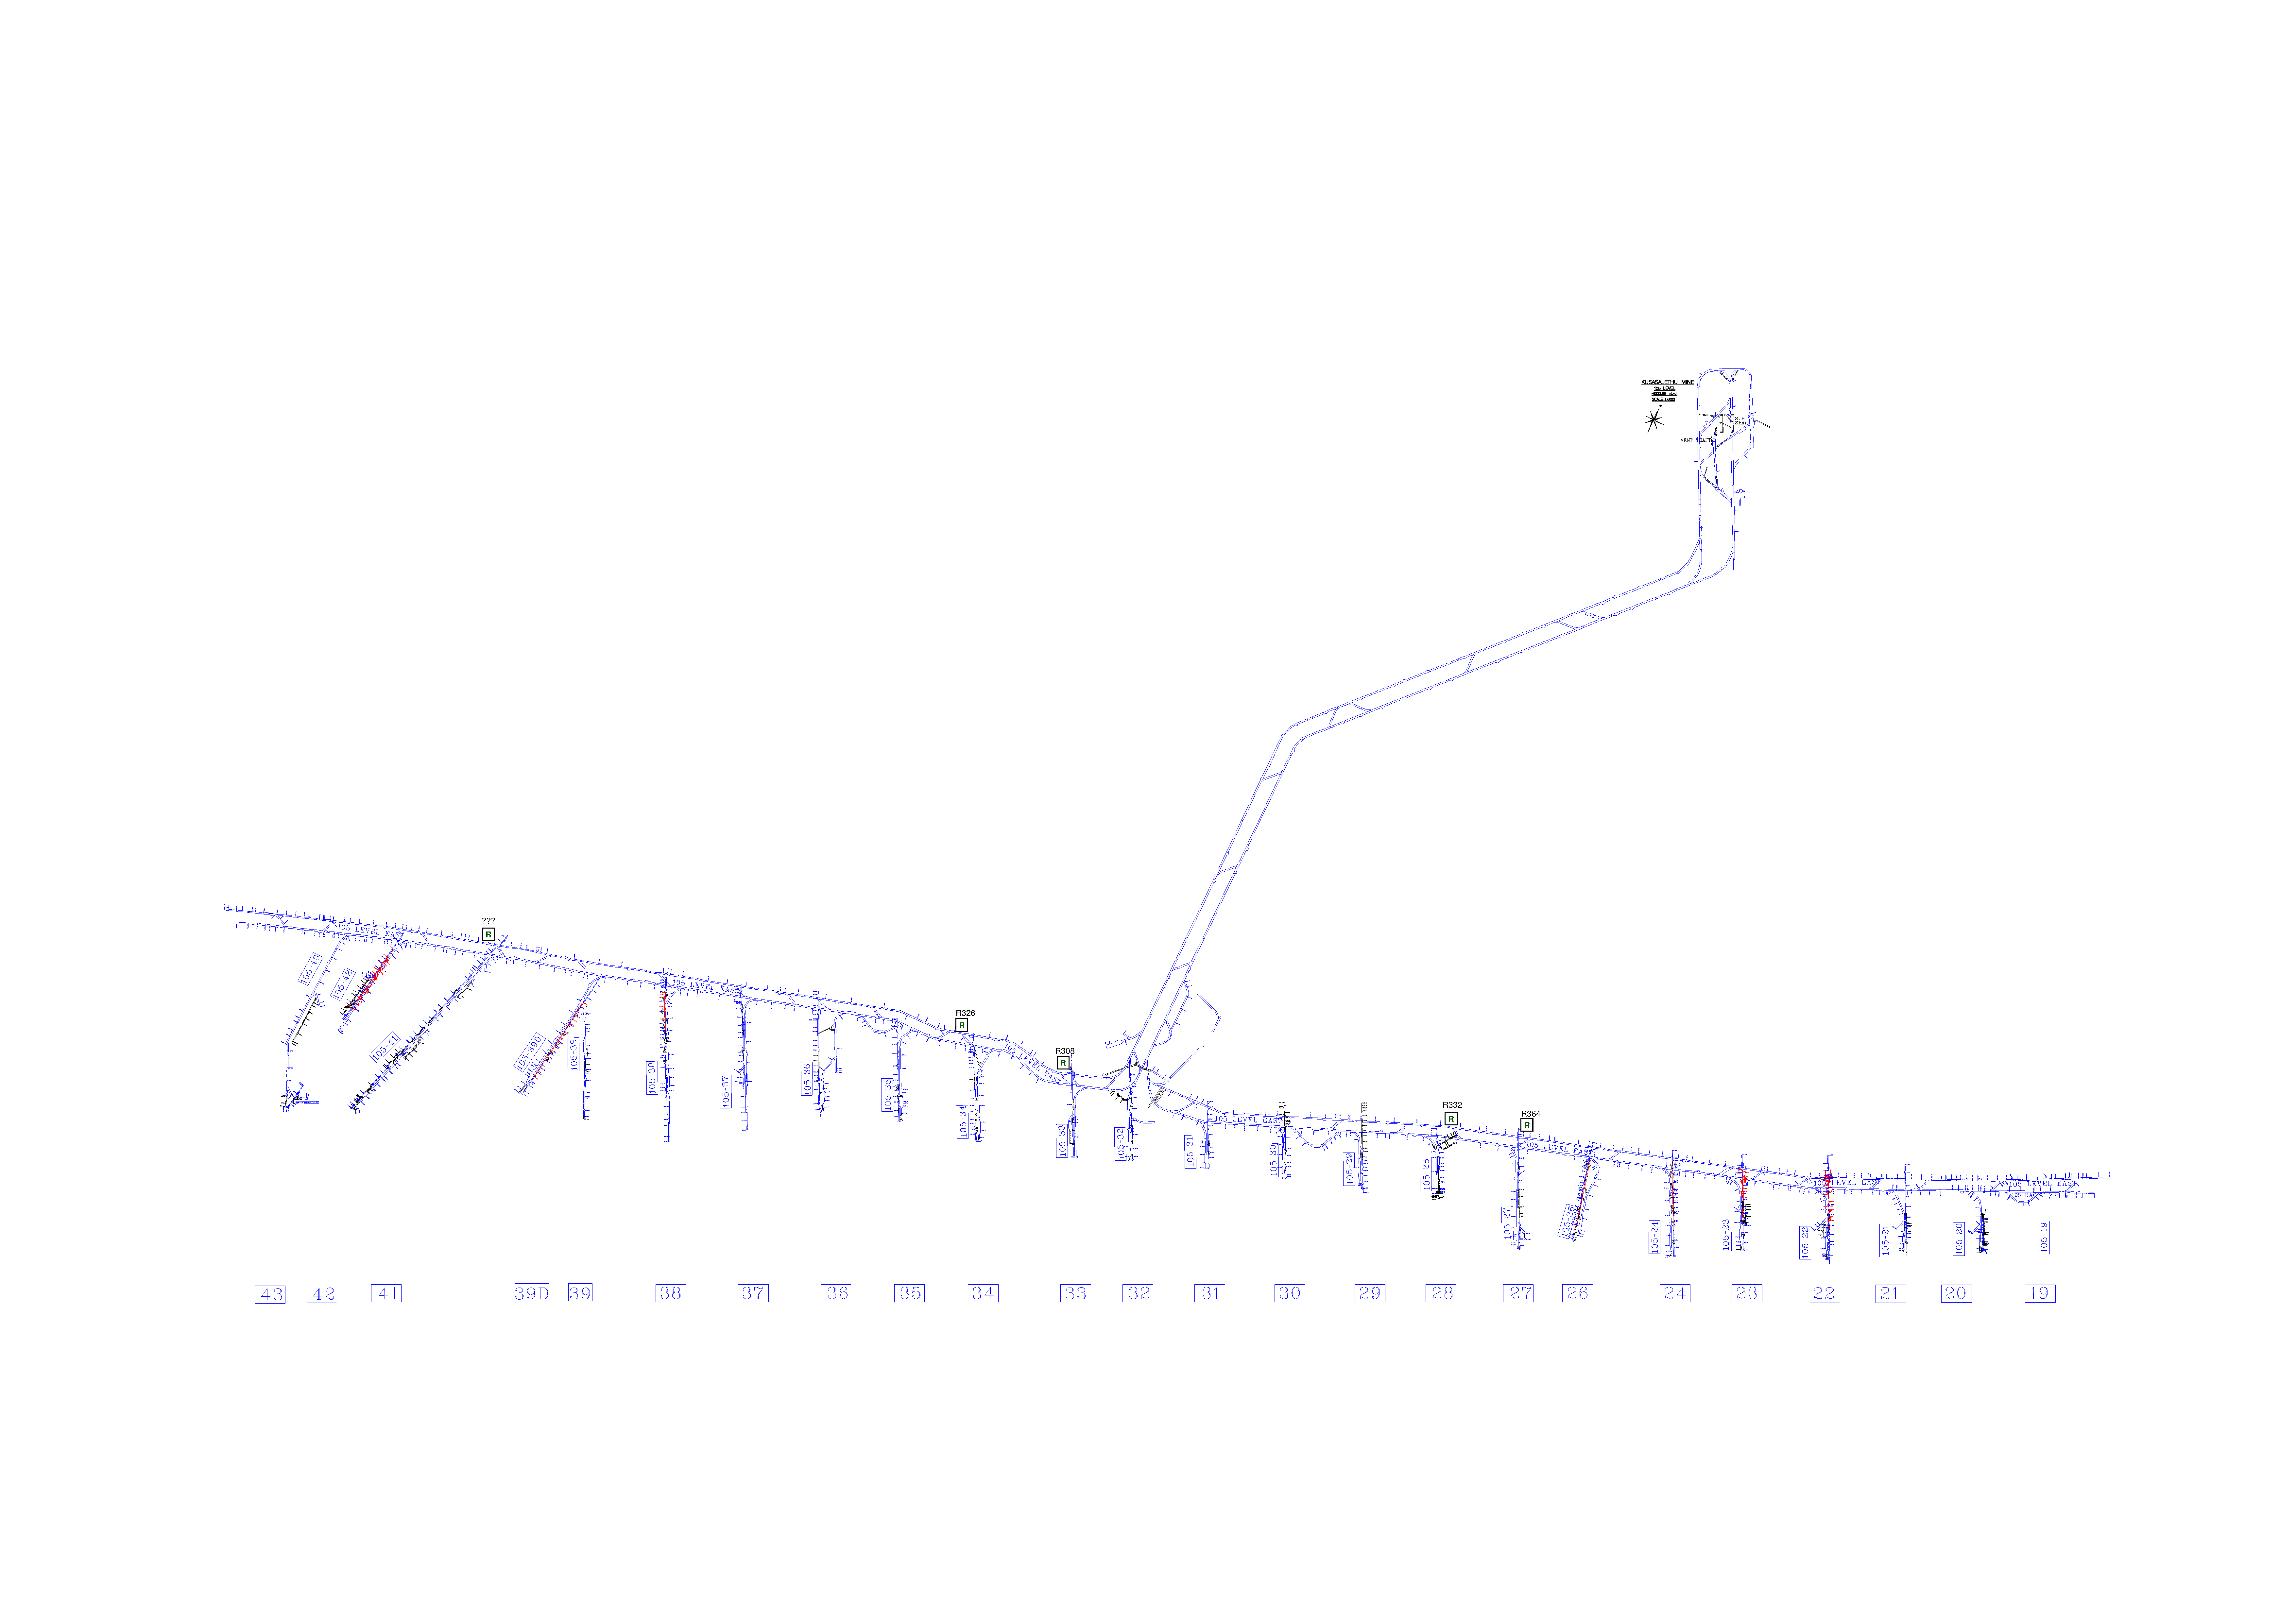
\includegraphics[trim =10cm 20cm 10cm 40cm, clip=true, width=\textwidth]{Graphs/4/LevelLayout/105L.pdf}}
		\caption{Underground level layout.}
		\label{fig: KUS Underground level layout}
	\end{figure}	
	\subsection{Model development}
	
	Using the data obtained from the investigation of the system, a  simulation model was developed in software. The modelling methodology described in Chapter 3 was then utilised to develop a model for the system. The entire model is shown in Appendix \ref{ASchematics} Figure \ref{fig: KUS Baseline model}. The model parameters were then calibrated to match the actual data from the mine.
	
	\subsubsection{Verification of baseline simulation}
	Verification of the model was performed firstly by comparing the simulation outputs to actual measured values. To simplify the model, the actual measured pressure is temporarily used as set points for the compressors. This ensured that the pressure in the network is identical to that of the actual measured system as shown in Figure \ref{fig: Verification Pressure kusasalethu}.
	
	\par 
	
	\begin{figure}[h]
		\centering
		\fbox{% GNUPLOT: LaTeX picture with Postscript
\begingroup
  \makeatletter
  \providecommand\color[2][]{%
    \GenericError{(gnuplot) \space\space\space\@spaces}{%
      Package color not loaded in conjunction with
      terminal option `colourtext'%
    }{See the gnuplot documentation for explanation.%
    }{Either use 'blacktext' in gnuplot or load the package
      color.sty in LaTeX.}%
    \renewcommand\color[2][]{}%
  }%
  \providecommand\includegraphics[2][]{%
    \GenericError{(gnuplot) \space\space\space\@spaces}{%
      Package graphicx or graphics not loaded%
    }{See the gnuplot documentation for explanation.%
    }{The gnuplot epslatex terminal needs graphicx.sty or graphics.sty.}%
    \renewcommand\includegraphics[2][]{}%
  }%
  \providecommand\rotatebox[2]{#2}%
  \@ifundefined{ifGPcolor}{%
    \newif\ifGPcolor
    \GPcolortrue
  }{}%
  \@ifundefined{ifGPblacktext}{%
    \newif\ifGPblacktext
    \GPblacktextfalse
  }{}%
  % define a \g@addto@macro without @ in the name:
  \let\gplgaddtomacro\g@addto@macro
  % define empty templates for all commands taking text:
  \gdef\gplbacktext{}%
  \gdef\gplfronttext{}%
  \makeatother
  \ifGPblacktext
    % no textcolor at all
    \def\colorrgb#1{}%
    \def\colorgray#1{}%
  \else
    % gray or color?
    \ifGPcolor
      \def\colorrgb#1{\color[rgb]{#1}}%
      \def\colorgray#1{\color[gray]{#1}}%
      \expandafter\def\csname LTw\endcsname{\color{white}}%
      \expandafter\def\csname LTb\endcsname{\color{black}}%
      \expandafter\def\csname LTa\endcsname{\color{black}}%
      \expandafter\def\csname LT0\endcsname{\color[rgb]{1,0,0}}%
      \expandafter\def\csname LT1\endcsname{\color[rgb]{0,1,0}}%
      \expandafter\def\csname LT2\endcsname{\color[rgb]{0,0,1}}%
      \expandafter\def\csname LT3\endcsname{\color[rgb]{1,0,1}}%
      \expandafter\def\csname LT4\endcsname{\color[rgb]{0,1,1}}%
      \expandafter\def\csname LT5\endcsname{\color[rgb]{1,1,0}}%
      \expandafter\def\csname LT6\endcsname{\color[rgb]{0,0,0}}%
      \expandafter\def\csname LT7\endcsname{\color[rgb]{1,0.3,0}}%
      \expandafter\def\csname LT8\endcsname{\color[rgb]{0.5,0.5,0.5}}%
    \else
      % gray
      \def\colorrgb#1{\color{black}}%
      \def\colorgray#1{\color[gray]{#1}}%
      \expandafter\def\csname LTw\endcsname{\color{white}}%
      \expandafter\def\csname LTb\endcsname{\color{black}}%
      \expandafter\def\csname LTa\endcsname{\color{black}}%
      \expandafter\def\csname LT0\endcsname{\color{black}}%
      \expandafter\def\csname LT1\endcsname{\color{black}}%
      \expandafter\def\csname LT2\endcsname{\color{black}}%
      \expandafter\def\csname LT3\endcsname{\color{black}}%
      \expandafter\def\csname LT4\endcsname{\color{black}}%
      \expandafter\def\csname LT5\endcsname{\color{black}}%
      \expandafter\def\csname LT6\endcsname{\color{black}}%
      \expandafter\def\csname LT7\endcsname{\color{black}}%
      \expandafter\def\csname LT8\endcsname{\color{black}}%
    \fi
  \fi
    \setlength{\unitlength}{0.0500bp}%
    \ifx\gptboxheight\undefined%
      \newlength{\gptboxheight}%
      \newlength{\gptboxwidth}%
      \newsavebox{\gptboxtext}%
    \fi%
    \setlength{\fboxrule}{0.5pt}%
    \setlength{\fboxsep}{1pt}%
\begin{picture}(9360.00,2772.00)%
    \gplgaddtomacro\gplbacktext{%
      \colorrgb{0.00,0.00,0.00}%
      \put(814,924){\makebox(0,0)[r]{\strut{}$300$}}%
      \colorrgb{0.00,0.00,0.00}%
      \put(814,1452){\makebox(0,0)[r]{\strut{}$350$}}%
      \colorrgb{0.00,0.00,0.00}%
      \put(814,1979){\makebox(0,0)[r]{\strut{}$400$}}%
      \colorrgb{0.00,0.00,0.00}%
      \put(814,2507){\makebox(0,0)[r]{\strut{}$450$}}%
      \colorrgb{0.00,0.00,0.00}%
      \put(946,704){\makebox(0,0){\strut{}00:00}}%
      \colorrgb{0.00,0.00,0.00}%
      \put(2157,704){\makebox(0,0){\strut{}04:00}}%
      \colorrgb{0.00,0.00,0.00}%
      \put(3369,704){\makebox(0,0){\strut{}08:00}}%
      \colorrgb{0.00,0.00,0.00}%
      \put(4580,704){\makebox(0,0){\strut{}12:00}}%
      \colorrgb{0.00,0.00,0.00}%
      \put(5791,704){\makebox(0,0){\strut{}16:00}}%
      \colorrgb{0.00,0.00,0.00}%
      \put(7003,704){\makebox(0,0){\strut{}20:00}}%
      \colorrgb{0.00,0.00,0.00}%
      \put(8214,704){\makebox(0,0){\strut{}00:00}}%
      \colorrgb{0.00,0.00,0.00}%
      \put(8346,924){\makebox(0,0)[l]{\strut{}$0$}}%
      \colorrgb{0.00,0.00,0.00}%
      \put(8346,1557){\makebox(0,0)[l]{\strut{}$10$}}%
      \colorrgb{0.00,0.00,0.00}%
      \put(8346,2190){\makebox(0,0)[l]{\strut{}$20$}}%
    }%
    \gplgaddtomacro\gplfronttext{%
      \csname LTb\endcsname%
      \put(176,1715){\rotatebox{-270}{\makebox(0,0){\strut{}Pressure $(kPa)$}}}%
      \put(8851,1715){\rotatebox{-270}{\makebox(0,0){\strut{}$\% error$}}}%
      \put(4580,374){\makebox(0,0){\strut{}Time of Day}}%
      \csname LTb\endcsname%
      \put(2241,173){\makebox(0,0)[r]{\strut{}Baseline press.}}%
      \csname LTb\endcsname%
      \put(5208,173){\makebox(0,0)[r]{\strut{}Simulated press.}}%
      \csname LTb\endcsname%
      \put(8175,173){\makebox(0,0)[r]{\strut{}Error}}%
    }%
    \gplbacktext
    \put(0,0){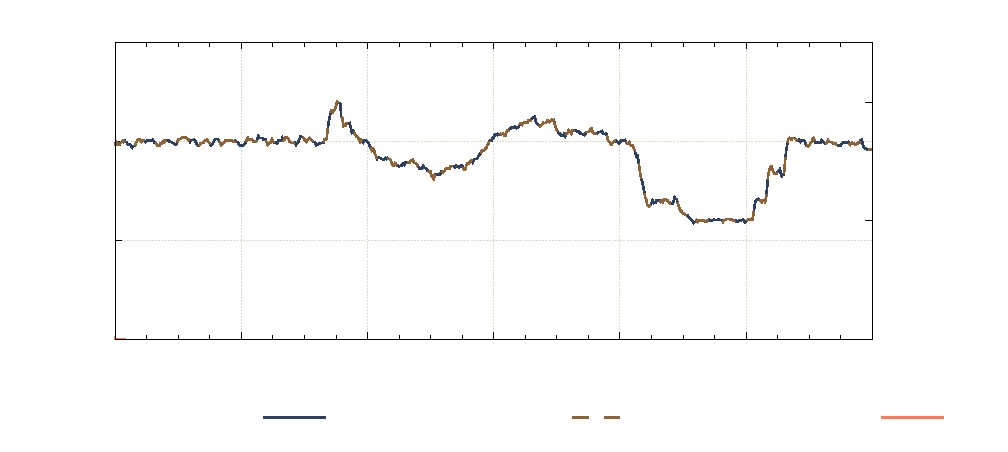
\includegraphics{Graphs/4/KusVerify/Pressure/Pressure}}%
    \gplfronttext
  \end{picture}%
\endgroup
}
		\caption{Comparing the pressure response of simulation to the actual measured pressure}
		\label{fig: Verification Pressure kusasalethu}
	\end{figure}

 	With the pressure set, the power and air flow outputs for components throughout the model were compared with their relative actual values. Figure \ref{fig: Verification Power kusasalethu} shows the comparison of the total power and flow of the system with the actual measure values for that same period. The accuracy for these parameters compared to the real system was $98.7 \%$ and $99.0 \%$ respectively. This was regarded as acceptable accuracy. 
 
	\begin{figure}[h]
		\centering
		\fbox{% GNUPLOT: LaTeX picture with Postscript
\begingroup
  \makeatletter
  \providecommand\color[2][]{%
    \GenericError{(gnuplot) \space\space\space\@spaces}{%
      Package color not loaded in conjunction with
      terminal option `colourtext'%
    }{See the gnuplot documentation for explanation.%
    }{Either use 'blacktext' in gnuplot or load the package
      color.sty in LaTeX.}%
    \renewcommand\color[2][]{}%
  }%
  \providecommand\includegraphics[2][]{%
    \GenericError{(gnuplot) \space\space\space\@spaces}{%
      Package graphicx or graphics not loaded%
    }{See the gnuplot documentation for explanation.%
    }{The gnuplot epslatex terminal needs graphicx.sty or graphics.sty.}%
    \renewcommand\includegraphics[2][]{}%
  }%
  \providecommand\rotatebox[2]{#2}%
  \@ifundefined{ifGPcolor}{%
    \newif\ifGPcolor
    \GPcolortrue
  }{}%
  \@ifundefined{ifGPblacktext}{%
    \newif\ifGPblacktext
    \GPblacktextfalse
  }{}%
  % define a \g@addto@macro without @ in the name:
  \let\gplgaddtomacro\g@addto@macro
  % define empty templates for all commands taking text:
  \gdef\gplbacktext{}%
  \gdef\gplfronttext{}%
  \makeatother
  \ifGPblacktext
    % no textcolor at all
    \def\colorrgb#1{}%
    \def\colorgray#1{}%
  \else
    % gray or color?
    \ifGPcolor
      \def\colorrgb#1{\color[rgb]{#1}}%
      \def\colorgray#1{\color[gray]{#1}}%
      \expandafter\def\csname LTw\endcsname{\color{white}}%
      \expandafter\def\csname LTb\endcsname{\color{black}}%
      \expandafter\def\csname LTa\endcsname{\color{black}}%
      \expandafter\def\csname LT0\endcsname{\color[rgb]{1,0,0}}%
      \expandafter\def\csname LT1\endcsname{\color[rgb]{0,1,0}}%
      \expandafter\def\csname LT2\endcsname{\color[rgb]{0,0,1}}%
      \expandafter\def\csname LT3\endcsname{\color[rgb]{1,0,1}}%
      \expandafter\def\csname LT4\endcsname{\color[rgb]{0,1,1}}%
      \expandafter\def\csname LT5\endcsname{\color[rgb]{1,1,0}}%
      \expandafter\def\csname LT6\endcsname{\color[rgb]{0,0,0}}%
      \expandafter\def\csname LT7\endcsname{\color[rgb]{1,0.3,0}}%
      \expandafter\def\csname LT8\endcsname{\color[rgb]{0.5,0.5,0.5}}%
    \else
      % gray
      \def\colorrgb#1{\color{black}}%
      \def\colorgray#1{\color[gray]{#1}}%
      \expandafter\def\csname LTw\endcsname{\color{white}}%
      \expandafter\def\csname LTb\endcsname{\color{black}}%
      \expandafter\def\csname LTa\endcsname{\color{black}}%
      \expandafter\def\csname LT0\endcsname{\color{black}}%
      \expandafter\def\csname LT1\endcsname{\color{black}}%
      \expandafter\def\csname LT2\endcsname{\color{black}}%
      \expandafter\def\csname LT3\endcsname{\color{black}}%
      \expandafter\def\csname LT4\endcsname{\color{black}}%
      \expandafter\def\csname LT5\endcsname{\color{black}}%
      \expandafter\def\csname LT6\endcsname{\color{black}}%
      \expandafter\def\csname LT7\endcsname{\color{black}}%
      \expandafter\def\csname LT8\endcsname{\color{black}}%
    \fi
  \fi
    \setlength{\unitlength}{0.0500bp}%
    \ifx\gptboxheight\undefined%
      \newlength{\gptboxheight}%
      \newlength{\gptboxwidth}%
      \newsavebox{\gptboxtext}%
    \fi%
    \setlength{\fboxrule}{0.5pt}%
    \setlength{\fboxsep}{1pt}%
\begin{picture}(9360.00,3276.00)%
    \gplgaddtomacro\gplbacktext{%
      \colorrgb{0.00,0.00,0.00}%
      \put(682,924){\makebox(0,0)[r]{\strut{}$30$}}%
      \colorrgb{0.00,0.00,0.00}%
      \put(682,1967){\makebox(0,0)[r]{\strut{}$40$}}%
      \colorrgb{0.00,0.00,0.00}%
      \put(682,3011){\makebox(0,0)[r]{\strut{}$50$}}%
      \colorrgb{0.00,0.00,0.00}%
      \put(814,704){\makebox(0,0){\strut{}00:00}}%
      \colorrgb{0.00,0.00,0.00}%
      \put(2047,704){\makebox(0,0){\strut{}04:00}}%
      \colorrgb{0.00,0.00,0.00}%
      \put(3281,704){\makebox(0,0){\strut{}08:00}}%
      \colorrgb{0.00,0.00,0.00}%
      \put(4514,704){\makebox(0,0){\strut{}12:00}}%
      \colorrgb{0.00,0.00,0.00}%
      \put(5747,704){\makebox(0,0){\strut{}16:00}}%
      \colorrgb{0.00,0.00,0.00}%
      \put(6981,704){\makebox(0,0){\strut{}20:00}}%
      \colorrgb{0.00,0.00,0.00}%
      \put(8214,704){\makebox(0,0){\strut{}00:00}}%
      \colorrgb{0.00,0.00,0.00}%
      \put(8346,924){\makebox(0,0)[l]{\strut{}$0$}}%
      \colorrgb{0.00,0.00,0.00}%
      \put(8346,1759){\makebox(0,0)[l]{\strut{}$10$}}%
      \colorrgb{0.00,0.00,0.00}%
      \put(8346,2594){\makebox(0,0)[l]{\strut{}$20$}}%
    }%
    \gplgaddtomacro\gplfronttext{%
      \csname LTb\endcsname%
      \put(176,1967){\rotatebox{-270}{\makebox(0,0){\strut{}flow $(kg/s)$}}}%
      \put(8851,1967){\rotatebox{-270}{\makebox(0,0){\strut{}$\% error$}}}%
      \put(4514,374){\makebox(0,0){\strut{}Time of Day}}%
      \csname LTb\endcsname%
      \put(2307,173){\makebox(0,0)[r]{\strut{}Baseline flow}}%
      \csname LTb\endcsname%
      \put(5010,173){\makebox(0,0)[r]{\strut{}Simulated flow}}%
      \csname LTb\endcsname%
      \put(7713,173){\makebox(0,0)[r]{\strut{}Error}}%
    }%
    \gplbacktext
    \put(0,0){\fbox{
\includegraphics[trim=0 0 0.1cm 0, clip]{Graphs/4/KusVerify/Flow/Flow}}}%
    \gplfronttext
  \end{picture}%
\endgroup
}
		(a)\\
		\fbox{% GNUPLOT: LaTeX picture with Postscript
\begingroup
  \makeatletter
  \providecommand\color[2][]{%
    \GenericError{(gnuplot) \space\space\space\@spaces}{%
      Package color not loaded in conjunction with
      terminal option `colourtext'%
    }{See the gnuplot documentation for explanation.%
    }{Either use 'blacktext' in gnuplot or load the package
      color.sty in LaTeX.}%
    \renewcommand\color[2][]{}%
  }%
  \providecommand\includegraphics[2][]{%
    \GenericError{(gnuplot) \space\space\space\@spaces}{%
      Package graphicx or graphics not loaded%
    }{See the gnuplot documentation for explanation.%
    }{The gnuplot epslatex terminal needs graphicx.sty or graphics.sty.}%
    \renewcommand\includegraphics[2][]{}%
  }%
  \providecommand\rotatebox[2]{#2}%
  \@ifundefined{ifGPcolor}{%
    \newif\ifGPcolor
    \GPcolortrue
  }{}%
  \@ifundefined{ifGPblacktext}{%
    \newif\ifGPblacktext
    \GPblacktextfalse
  }{}%
  % define a \g@addto@macro without @ in the name:
  \let\gplgaddtomacro\g@addto@macro
  % define empty templates for all commands taking text:
  \gdef\gplbacktext{}%
  \gdef\gplfronttext{}%
  \makeatother
  \ifGPblacktext
    % no textcolor at all
    \def\colorrgb#1{}%
    \def\colorgray#1{}%
  \else
    % gray or color?
    \ifGPcolor
      \def\colorrgb#1{\color[rgb]{#1}}%
      \def\colorgray#1{\color[gray]{#1}}%
      \expandafter\def\csname LTw\endcsname{\color{white}}%
      \expandafter\def\csname LTb\endcsname{\color{black}}%
      \expandafter\def\csname LTa\endcsname{\color{black}}%
      \expandafter\def\csname LT0\endcsname{\color[rgb]{1,0,0}}%
      \expandafter\def\csname LT1\endcsname{\color[rgb]{0,1,0}}%
      \expandafter\def\csname LT2\endcsname{\color[rgb]{0,0,1}}%
      \expandafter\def\csname LT3\endcsname{\color[rgb]{1,0,1}}%
      \expandafter\def\csname LT4\endcsname{\color[rgb]{0,1,1}}%
      \expandafter\def\csname LT5\endcsname{\color[rgb]{1,1,0}}%
      \expandafter\def\csname LT6\endcsname{\color[rgb]{0,0,0}}%
      \expandafter\def\csname LT7\endcsname{\color[rgb]{1,0.3,0}}%
      \expandafter\def\csname LT8\endcsname{\color[rgb]{0.5,0.5,0.5}}%
    \else
      % gray
      \def\colorrgb#1{\color{black}}%
      \def\colorgray#1{\color[gray]{#1}}%
      \expandafter\def\csname LTw\endcsname{\color{white}}%
      \expandafter\def\csname LTb\endcsname{\color{black}}%
      \expandafter\def\csname LTa\endcsname{\color{black}}%
      \expandafter\def\csname LT0\endcsname{\color{black}}%
      \expandafter\def\csname LT1\endcsname{\color{black}}%
      \expandafter\def\csname LT2\endcsname{\color{black}}%
      \expandafter\def\csname LT3\endcsname{\color{black}}%
      \expandafter\def\csname LT4\endcsname{\color{black}}%
      \expandafter\def\csname LT5\endcsname{\color{black}}%
      \expandafter\def\csname LT6\endcsname{\color{black}}%
      \expandafter\def\csname LT7\endcsname{\color{black}}%
      \expandafter\def\csname LT8\endcsname{\color{black}}%
    \fi
  \fi
    \setlength{\unitlength}{0.0500bp}%
    \ifx\gptboxheight\undefined%
      \newlength{\gptboxheight}%
      \newlength{\gptboxwidth}%
      \newsavebox{\gptboxtext}%
    \fi%
    \setlength{\fboxrule}{0.5pt}%
    \setlength{\fboxsep}{1pt}%
\begin{picture}(9360.00,3276.00)%
    \gplgaddtomacro\gplbacktext{%
      \colorrgb{0.00,0.00,0.00}%
      \put(682,924){\makebox(0,0)[r]{\strut{}$8$}}%
      \colorrgb{0.00,0.00,0.00}%
      \put(682,1222){\makebox(0,0)[r]{\strut{}$9$}}%
      \colorrgb{0.00,0.00,0.00}%
      \put(682,1520){\makebox(0,0)[r]{\strut{}$10$}}%
      \colorrgb{0.00,0.00,0.00}%
      \put(682,1818){\makebox(0,0)[r]{\strut{}$11$}}%
      \colorrgb{0.00,0.00,0.00}%
      \put(682,2117){\makebox(0,0)[r]{\strut{}$12$}}%
      \colorrgb{0.00,0.00,0.00}%
      \put(682,2415){\makebox(0,0)[r]{\strut{}$13$}}%
      \colorrgb{0.00,0.00,0.00}%
      \put(682,2713){\makebox(0,0)[r]{\strut{}$14$}}%
      \colorrgb{0.00,0.00,0.00}%
      \put(682,3011){\makebox(0,0)[r]{\strut{}$15$}}%
      \colorrgb{0.00,0.00,0.00}%
      \put(814,704){\makebox(0,0){\strut{}00:00}}%
      \colorrgb{0.00,0.00,0.00}%
      \put(2047,704){\makebox(0,0){\strut{}04:00}}%
      \colorrgb{0.00,0.00,0.00}%
      \put(3281,704){\makebox(0,0){\strut{}08:00}}%
      \colorrgb{0.00,0.00,0.00}%
      \put(4514,704){\makebox(0,0){\strut{}12:00}}%
      \colorrgb{0.00,0.00,0.00}%
      \put(5747,704){\makebox(0,0){\strut{}16:00}}%
      \colorrgb{0.00,0.00,0.00}%
      \put(6981,704){\makebox(0,0){\strut{}20:00}}%
      \colorrgb{0.00,0.00,0.00}%
      \put(8214,704){\makebox(0,0){\strut{}00:00}}%
      \colorrgb{0.00,0.00,0.00}%
      \put(8346,924){\makebox(0,0)[l]{\strut{}$0$}}%
      \colorrgb{0.00,0.00,0.00}%
      \put(8346,1759){\makebox(0,0)[l]{\strut{}$10$}}%
      \colorrgb{0.00,0.00,0.00}%
      \put(8346,2594){\makebox(0,0)[l]{\strut{}$20$}}%
    }%
    \gplgaddtomacro\gplfronttext{%
      \csname LTb\endcsname%
      \put(176,1967){\rotatebox{-270}{\makebox(0,0){\strut{}Power $(MW)$}}}%
      \put(8851,1967){\rotatebox{-270}{\makebox(0,0){\strut{}$\% error$}}}%
      \put(4514,374){\makebox(0,0){\strut{}Time of Day}}%
      \csname LTb\endcsname%
      \put(2241,173){\makebox(0,0)[r]{\strut{}Baseline power}}%
      \csname LTb\endcsname%
      \put(5076,173){\makebox(0,0)[r]{\strut{}Simulated power}}%
      \csname LTb\endcsname%
      \put(7911,173){\makebox(0,0)[r]{\strut{}Error}}%
    }%
    \gplbacktext
    \put(0,0){\fbox{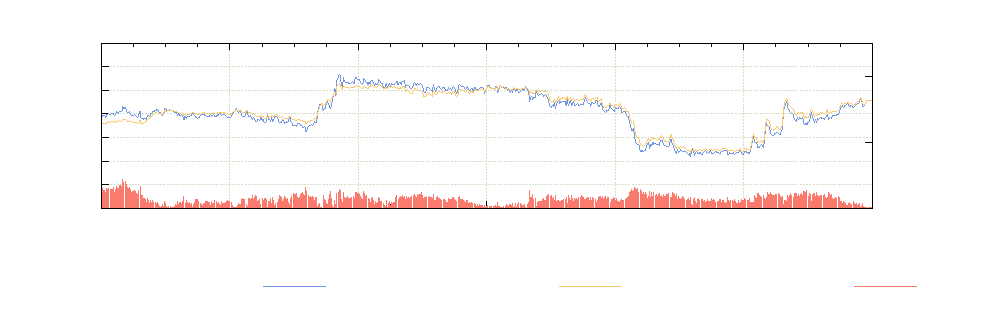
\includegraphics[trim=0 0 0.1cm 0, clip]{Graphs/4/KusVerify/Power/Power}}}%
    \gplfronttext
  \end{picture}%
\endgroup
}
		(b)\\
		\caption{Verification of the total (a) flow and (b) power of the system using the actual pressure profile.}
		\label{fig: Verification Power kusasalethu}
	\end{figure}

	Once all the power and flow parameters were checked calibrated with minimal error, the systems response to the pressure set-points was checked. The compressor models were replaced with the pressure set-point profile instead of the measured outlet pressure profile. The simulated outlet pressure was then compared to the actual measured outlet, this is shown in Figure \ref{fig: Verification Pressure kusasalethu Setpoint}.

	\begin{figure}[h]
		\centering
		\fbox{% GNUPLOT: LaTeX picture with Postscript
\begingroup
  \makeatletter
  \providecommand\color[2][]{%
    \GenericError{(gnuplot) \space\space\space\@spaces}{%
      Package color not loaded in conjunction with
      terminal option `colourtext'%
    }{See the gnuplot documentation for explanation.%
    }{Either use 'blacktext' in gnuplot or load the package
      color.sty in LaTeX.}%
    \renewcommand\color[2][]{}%
  }%
  \providecommand\includegraphics[2][]{%
    \GenericError{(gnuplot) \space\space\space\@spaces}{%
      Package graphicx or graphics not loaded%
    }{See the gnuplot documentation for explanation.%
    }{The gnuplot epslatex terminal needs graphicx.sty or graphics.sty.}%
    \renewcommand\includegraphics[2][]{}%
  }%
  \providecommand\rotatebox[2]{#2}%
  \@ifundefined{ifGPcolor}{%
    \newif\ifGPcolor
    \GPcolortrue
  }{}%
  \@ifundefined{ifGPblacktext}{%
    \newif\ifGPblacktext
    \GPblacktextfalse
  }{}%
  % define a \g@addto@macro without @ in the name:
  \let\gplgaddtomacro\g@addto@macro
  % define empty templates for all commands taking text:
  \gdef\gplbacktext{}%
  \gdef\gplfronttext{}%
  \makeatother
  \ifGPblacktext
    % no textcolor at all
    \def\colorrgb#1{}%
    \def\colorgray#1{}%
  \else
    % gray or color?
    \ifGPcolor
      \def\colorrgb#1{\color[rgb]{#1}}%
      \def\colorgray#1{\color[gray]{#1}}%
      \expandafter\def\csname LTw\endcsname{\color{white}}%
      \expandafter\def\csname LTb\endcsname{\color{black}}%
      \expandafter\def\csname LTa\endcsname{\color{black}}%
      \expandafter\def\csname LT0\endcsname{\color[rgb]{1,0,0}}%
      \expandafter\def\csname LT1\endcsname{\color[rgb]{0,1,0}}%
      \expandafter\def\csname LT2\endcsname{\color[rgb]{0,0,1}}%
      \expandafter\def\csname LT3\endcsname{\color[rgb]{1,0,1}}%
      \expandafter\def\csname LT4\endcsname{\color[rgb]{0,1,1}}%
      \expandafter\def\csname LT5\endcsname{\color[rgb]{1,1,0}}%
      \expandafter\def\csname LT6\endcsname{\color[rgb]{0,0,0}}%
      \expandafter\def\csname LT7\endcsname{\color[rgb]{1,0.3,0}}%
      \expandafter\def\csname LT8\endcsname{\color[rgb]{0.5,0.5,0.5}}%
    \else
      % gray
      \def\colorrgb#1{\color{black}}%
      \def\colorgray#1{\color[gray]{#1}}%
      \expandafter\def\csname LTw\endcsname{\color{white}}%
      \expandafter\def\csname LTb\endcsname{\color{black}}%
      \expandafter\def\csname LTa\endcsname{\color{black}}%
      \expandafter\def\csname LT0\endcsname{\color{black}}%
      \expandafter\def\csname LT1\endcsname{\color{black}}%
      \expandafter\def\csname LT2\endcsname{\color{black}}%
      \expandafter\def\csname LT3\endcsname{\color{black}}%
      \expandafter\def\csname LT4\endcsname{\color{black}}%
      \expandafter\def\csname LT5\endcsname{\color{black}}%
      \expandafter\def\csname LT6\endcsname{\color{black}}%
      \expandafter\def\csname LT7\endcsname{\color{black}}%
      \expandafter\def\csname LT8\endcsname{\color{black}}%
    \fi
  \fi
    \setlength{\unitlength}{0.0500bp}%
    \ifx\gptboxheight\undefined%
      \newlength{\gptboxheight}%
      \newlength{\gptboxwidth}%
      \newsavebox{\gptboxtext}%
    \fi%
    \setlength{\fboxrule}{0.5pt}%
    \setlength{\fboxsep}{1pt}%
\begin{picture}(9360.00,4032.00)%
    \gplgaddtomacro\gplbacktext{%
      \colorrgb{0.00,0.00,0.00}%
      \put(814,1144){\makebox(0,0)[r]{\strut{}$300$}}%
      \colorrgb{0.00,0.00,0.00}%
      \put(814,2018){\makebox(0,0)[r]{\strut{}$350$}}%
      \colorrgb{0.00,0.00,0.00}%
      \put(814,2893){\makebox(0,0)[r]{\strut{}$400$}}%
      \colorrgb{0.00,0.00,0.00}%
      \put(814,3767){\makebox(0,0)[r]{\strut{}$450$}}%
      \colorrgb{0.00,0.00,0.00}%
      \put(946,924){\makebox(0,0){\strut{}00:00}}%
      \colorrgb{0.00,0.00,0.00}%
      \put(2157,924){\makebox(0,0){\strut{}04:00}}%
      \colorrgb{0.00,0.00,0.00}%
      \put(3369,924){\makebox(0,0){\strut{}08:00}}%
      \colorrgb{0.00,0.00,0.00}%
      \put(4580,924){\makebox(0,0){\strut{}12:00}}%
      \colorrgb{0.00,0.00,0.00}%
      \put(5791,924){\makebox(0,0){\strut{}16:00}}%
      \colorrgb{0.00,0.00,0.00}%
      \put(7003,924){\makebox(0,0){\strut{}20:00}}%
      \colorrgb{0.00,0.00,0.00}%
      \put(8214,924){\makebox(0,0){\strut{}00:00}}%
      \colorrgb{0.00,0.00,0.00}%
      \put(8346,1144){\makebox(0,0)[l]{\strut{}$0$}}%
      \colorrgb{0.00,0.00,0.00}%
      \put(8346,2193){\makebox(0,0)[l]{\strut{}$10$}}%
      \colorrgb{0.00,0.00,0.00}%
      \put(8346,3242){\makebox(0,0)[l]{\strut{}$20$}}%
    }%
    \gplgaddtomacro\gplfronttext{%
      \csname LTb\endcsname%
      \put(176,2455){\rotatebox{-270}{\makebox(0,0){\strut{}Pressure $(kPa)$}}}%
      \put(8851,2455){\rotatebox{-270}{\makebox(0,0){\strut{}$\% error$}}}%
      \put(4580,594){\makebox(0,0){\strut{}Time of Day}}%
      \csname LTb\endcsname%
      \put(3725,393){\makebox(0,0)[r]{\strut{}Actual}}%
      \csname LTb\endcsname%
      \put(3725,173){\makebox(0,0)[r]{\strut{}Simulation.}}%
      \csname LTb\endcsname%
      \put(6032,393){\makebox(0,0)[r]{\strut{}Set-point}}%
      \csname LTb\endcsname%
      \put(5900,173){\makebox(0,0)[r]{\strut{}Rel. Error}}%
    }%
    \gplbacktext
    \put(0,0){\fbox{
\includegraphics[trim=0 0 0.1cm 0, clip]{Graphs/4/KusVerify/Pressure2/Pressure2}}}%
    \gplfronttext
  \end{picture}%
\endgroup
}
		\caption{Verifying the Pressure response of the system give the pressure set points as inputs}
		\label{fig: Verification Pressure kusasalethu Setpoint}
	\end{figure}
	\par 
	It was noted the during peak air usage periods, between 07:00 and 13:00, that the outlet pressure dropped well below the desired set-point. This was because the compressors struggled to keep up with the air demand during those periods, resulting in a pressure lower than the desired set-point. This was reproduced in the simulation.
	\subsection{Scenario 1. Refuge bay optimisation}
	From investigations that were conducted on the mines compressed system, unnecessary refuge bay leaks was identified as a significant inefficiency that can be reduced. Early tests on a single mining level indicated that a reduction refuge bay leaks, by closing the valves would lead to a air saving of $0.05$ $kg/s$ per refuge bay at typical operational pressures. This measurement was conservative as not all of the refuge bays on the level could be closed for the test.
	\par 
	Further tests, integrating more refuge bays for a longer period would not be possible without buy in from the mine's management. To gain this buy-in, the potential financial and operational benefits of refuge bay leakage interventions would first need to be quantified. A simulation model was hence developed to accurately estimate the savings for any interventions.
	\par
	Refuge bay components were added to the baseline modelled discussed previously. Using the test results, refuge bay leaks were added to the simulation model. \gls{scada} data was used to verify the new baseline simulation model with an accuracy of 98\%. Using the per-level layouts obtained from the investigation the location and number of refuge bay components were identified. The full simulation model is shown in Figure \ref{fig: Refuge bay layout} in Appendix \ref{ASchematics}.
	\par 
	
	\begin{figure}[h]
		\centering
		\fbox{% GNUPLOT: LaTeX picture with Postscript
\begingroup
  \makeatletter
  \providecommand\color[2][]{%
    \GenericError{(gnuplot) \space\space\space\@spaces}{%
      Package color not loaded in conjunction with
      terminal option `colourtext'%
    }{See the gnuplot documentation for explanation.%
    }{Either use 'blacktext' in gnuplot or load the package
      color.sty in LaTeX.}%
    \renewcommand\color[2][]{}%
  }%
  \providecommand\includegraphics[2][]{%
    \GenericError{(gnuplot) \space\space\space\@spaces}{%
      Package graphicx or graphics not loaded%
    }{See the gnuplot documentation for explanation.%
    }{The gnuplot epslatex terminal needs graphicx.sty or graphics.sty.}%
    \renewcommand\includegraphics[2][]{}%
  }%
  \providecommand\rotatebox[2]{#2}%
  \@ifundefined{ifGPcolor}{%
    \newif\ifGPcolor
    \GPcolortrue
  }{}%
  \@ifundefined{ifGPblacktext}{%
    \newif\ifGPblacktext
    \GPblacktextfalse
  }{}%
  % define a \g@addto@macro without @ in the name:
  \let\gplgaddtomacro\g@addto@macro
  % define empty templates for all commands taking text:
  \gdef\gplbacktext{}%
  \gdef\gplfronttext{}%
  \makeatother
  \ifGPblacktext
    % no textcolor at all
    \def\colorrgb#1{}%
    \def\colorgray#1{}%
  \else
    % gray or color?
    \ifGPcolor
      \def\colorrgb#1{\color[rgb]{#1}}%
      \def\colorgray#1{\color[gray]{#1}}%
      \expandafter\def\csname LTw\endcsname{\color{white}}%
      \expandafter\def\csname LTb\endcsname{\color{black}}%
      \expandafter\def\csname LTa\endcsname{\color{black}}%
      \expandafter\def\csname LT0\endcsname{\color[rgb]{1,0,0}}%
      \expandafter\def\csname LT1\endcsname{\color[rgb]{0,1,0}}%
      \expandafter\def\csname LT2\endcsname{\color[rgb]{0,0,1}}%
      \expandafter\def\csname LT3\endcsname{\color[rgb]{1,0,1}}%
      \expandafter\def\csname LT4\endcsname{\color[rgb]{0,1,1}}%
      \expandafter\def\csname LT5\endcsname{\color[rgb]{1,1,0}}%
      \expandafter\def\csname LT6\endcsname{\color[rgb]{0,0,0}}%
      \expandafter\def\csname LT7\endcsname{\color[rgb]{1,0.3,0}}%
      \expandafter\def\csname LT8\endcsname{\color[rgb]{0.5,0.5,0.5}}%
    \else
      % gray
      \def\colorrgb#1{\color{black}}%
      \def\colorgray#1{\color[gray]{#1}}%
      \expandafter\def\csname LTw\endcsname{\color{white}}%
      \expandafter\def\csname LTb\endcsname{\color{black}}%
      \expandafter\def\csname LTa\endcsname{\color{black}}%
      \expandafter\def\csname LT0\endcsname{\color{black}}%
      \expandafter\def\csname LT1\endcsname{\color{black}}%
      \expandafter\def\csname LT2\endcsname{\color{black}}%
      \expandafter\def\csname LT3\endcsname{\color{black}}%
      \expandafter\def\csname LT4\endcsname{\color{black}}%
      \expandafter\def\csname LT5\endcsname{\color{black}}%
      \expandafter\def\csname LT6\endcsname{\color{black}}%
      \expandafter\def\csname LT7\endcsname{\color{black}}%
      \expandafter\def\csname LT8\endcsname{\color{black}}%
    \fi
  \fi
    \setlength{\unitlength}{0.0500bp}%
    \ifx\gptboxheight\undefined%
      \newlength{\gptboxheight}%
      \newlength{\gptboxwidth}%
      \newsavebox{\gptboxtext}%
    \fi%
    \setlength{\fboxrule}{0.5pt}%
    \setlength{\fboxsep}{1pt}%
\begin{picture}(9360.00,3780.00)%
    \gplgaddtomacro\gplbacktext{%
      \colorrgb{0.00,0.00,0.00}%
      \put(682,924){\makebox(0,0)[r]{\strut{}$0$}}%
      \colorrgb{0.00,0.00,0.00}%
      \put(682,1788){\makebox(0,0)[r]{\strut{}$5$}}%
      \colorrgb{0.00,0.00,0.00}%
      \put(682,2651){\makebox(0,0)[r]{\strut{}$10$}}%
      \colorrgb{0.00,0.00,0.00}%
      \put(682,3515){\makebox(0,0)[r]{\strut{}$15$}}%
      \colorrgb{0.00,0.00,0.00}%
      \put(814,704){\makebox(0,0){\strut{}00:00}}%
      \colorrgb{0.00,0.00,0.00}%
      \put(2172,704){\makebox(0,0){\strut{}04:00}}%
      \colorrgb{0.00,0.00,0.00}%
      \put(3530,704){\makebox(0,0){\strut{}08:00}}%
      \colorrgb{0.00,0.00,0.00}%
      \put(4888,704){\makebox(0,0){\strut{}12:00}}%
      \colorrgb{0.00,0.00,0.00}%
      \put(6246,704){\makebox(0,0){\strut{}16:00}}%
      \colorrgb{0.00,0.00,0.00}%
      \put(7604,704){\makebox(0,0){\strut{}20:00}}%
      \colorrgb{0.00,0.00,0.00}%
      \put(8962,704){\makebox(0,0){\strut{}00:00}}%
    }%
    \gplgaddtomacro\gplfronttext{%
      \csname LTb\endcsname%
      \put(176,2219){\rotatebox{-270}{\makebox(0,0){\strut{}Power $(MW)$}}}%
      \put(4888,374){\makebox(0,0){\strut{}Time of Day}}%
      \csname LTb\endcsname%
      \put(2813,173){\makebox(0,0)[r]{\strut{}Baseline}}%
      \csname LTb\endcsname%
      \put(5252,173){\makebox(0,0)[r]{\strut{}Intervention}}%
      \csname LTb\endcsname%
      \put(7691,173){\makebox(0,0)[r]{\strut{}Power saving}}%
    }%
    \gplbacktext
    \put(0,0){
\includegraphics{Graphs/4/KUSResults/RefugePower/RefugePower}}%
    \gplfronttext
  \end{picture}%
\endgroup
}
		\caption{The Baseline system power compared to the system power when refuge bay leaks are reduce.}
		\label{fig: RefugeBay Power.}
	\end{figure}   

	\begin{figure}[h]
		\centering
		\fbox{% GNUPLOT: LaTeX picture with Postscript
\begingroup
  \makeatletter
  \providecommand\color[2][]{%
    \GenericError{(gnuplot) \space\space\space\@spaces}{%
      Package color not loaded in conjunction with
      terminal option `colourtext'%
    }{See the gnuplot documentation for explanation.%
    }{Either use 'blacktext' in gnuplot or load the package
      color.sty in LaTeX.}%
    \renewcommand\color[2][]{}%
  }%
  \providecommand\includegraphics[2][]{%
    \GenericError{(gnuplot) \space\space\space\@spaces}{%
      Package graphicx or graphics not loaded%
    }{See the gnuplot documentation for explanation.%
    }{The gnuplot epslatex terminal needs graphicx.sty or graphics.sty.}%
    \renewcommand\includegraphics[2][]{}%
  }%
  \providecommand\rotatebox[2]{#2}%
  \@ifundefined{ifGPcolor}{%
    \newif\ifGPcolor
    \GPcolortrue
  }{}%
  \@ifundefined{ifGPblacktext}{%
    \newif\ifGPblacktext
    \GPblacktextfalse
  }{}%
  % define a \g@addto@macro without @ in the name:
  \let\gplgaddtomacro\g@addto@macro
  % define empty templates for all commands taking text:
  \gdef\gplbacktext{}%
  \gdef\gplfronttext{}%
  \makeatother
  \ifGPblacktext
    % no textcolor at all
    \def\colorrgb#1{}%
    \def\colorgray#1{}%
  \else
    % gray or color?
    \ifGPcolor
      \def\colorrgb#1{\color[rgb]{#1}}%
      \def\colorgray#1{\color[gray]{#1}}%
      \expandafter\def\csname LTw\endcsname{\color{white}}%
      \expandafter\def\csname LTb\endcsname{\color{black}}%
      \expandafter\def\csname LTa\endcsname{\color{black}}%
      \expandafter\def\csname LT0\endcsname{\color[rgb]{1,0,0}}%
      \expandafter\def\csname LT1\endcsname{\color[rgb]{0,1,0}}%
      \expandafter\def\csname LT2\endcsname{\color[rgb]{0,0,1}}%
      \expandafter\def\csname LT3\endcsname{\color[rgb]{1,0,1}}%
      \expandafter\def\csname LT4\endcsname{\color[rgb]{0,1,1}}%
      \expandafter\def\csname LT5\endcsname{\color[rgb]{1,1,0}}%
      \expandafter\def\csname LT6\endcsname{\color[rgb]{0,0,0}}%
      \expandafter\def\csname LT7\endcsname{\color[rgb]{1,0.3,0}}%
      \expandafter\def\csname LT8\endcsname{\color[rgb]{0.5,0.5,0.5}}%
    \else
      % gray
      \def\colorrgb#1{\color{black}}%
      \def\colorgray#1{\color[gray]{#1}}%
      \expandafter\def\csname LTw\endcsname{\color{white}}%
      \expandafter\def\csname LTb\endcsname{\color{black}}%
      \expandafter\def\csname LTa\endcsname{\color{black}}%
      \expandafter\def\csname LT0\endcsname{\color{black}}%
      \expandafter\def\csname LT1\endcsname{\color{black}}%
      \expandafter\def\csname LT2\endcsname{\color{black}}%
      \expandafter\def\csname LT3\endcsname{\color{black}}%
      \expandafter\def\csname LT4\endcsname{\color{black}}%
      \expandafter\def\csname LT5\endcsname{\color{black}}%
      \expandafter\def\csname LT6\endcsname{\color{black}}%
      \expandafter\def\csname LT7\endcsname{\color{black}}%
      \expandafter\def\csname LT8\endcsname{\color{black}}%
    \fi
  \fi
    \setlength{\unitlength}{0.0500bp}%
    \ifx\gptboxheight\undefined%
      \newlength{\gptboxheight}%
      \newlength{\gptboxwidth}%
      \newsavebox{\gptboxtext}%
    \fi%
    \setlength{\fboxrule}{0.5pt}%
    \setlength{\fboxsep}{1pt}%
\begin{picture}(9360.00,3780.00)%
    \gplgaddtomacro\gplbacktext{%
      \colorrgb{0.00,0.00,0.00}%
      \put(814,1183){\makebox(0,0)[r]{\strut{}$360$}}%
      \colorrgb{0.00,0.00,0.00}%
      \put(814,1701){\makebox(0,0)[r]{\strut{}$380$}}%
      \colorrgb{0.00,0.00,0.00}%
      \put(814,2220){\makebox(0,0)[r]{\strut{}$400$}}%
      \colorrgb{0.00,0.00,0.00}%
      \put(814,2738){\makebox(0,0)[r]{\strut{}$420$}}%
      \colorrgb{0.00,0.00,0.00}%
      \put(814,3256){\makebox(0,0)[r]{\strut{}$440$}}%
      \colorrgb{0.00,0.00,0.00}%
      \put(946,704){\makebox(0,0){\strut{}00:00}}%
      \colorrgb{0.00,0.00,0.00}%
      \put(2282,704){\makebox(0,0){\strut{}04:00}}%
      \colorrgb{0.00,0.00,0.00}%
      \put(3618,704){\makebox(0,0){\strut{}08:00}}%
      \colorrgb{0.00,0.00,0.00}%
      \put(4954,704){\makebox(0,0){\strut{}12:00}}%
      \colorrgb{0.00,0.00,0.00}%
      \put(6290,704){\makebox(0,0){\strut{}16:00}}%
      \colorrgb{0.00,0.00,0.00}%
      \put(7626,704){\makebox(0,0){\strut{}20:00}}%
      \colorrgb{0.00,0.00,0.00}%
      \put(8962,704){\makebox(0,0){\strut{}00:00}}%
    }%
    \gplgaddtomacro\gplfronttext{%
      \csname LTb\endcsname%
      \put(176,2219){\rotatebox{-270}{\makebox(0,0){\strut{}Pressure $(kPa)$}}}%
      \put(4954,374){\makebox(0,0){\strut{}Time of Day}}%
      \csname LTb\endcsname%
      \put(4099,173){\makebox(0,0)[r]{\strut{}Baseline}}%
      \csname LTb\endcsname%
      \put(6538,173){\makebox(0,0)[r]{\strut{}Intervention}}%
    }%
    \gplbacktext
    \put(0,0){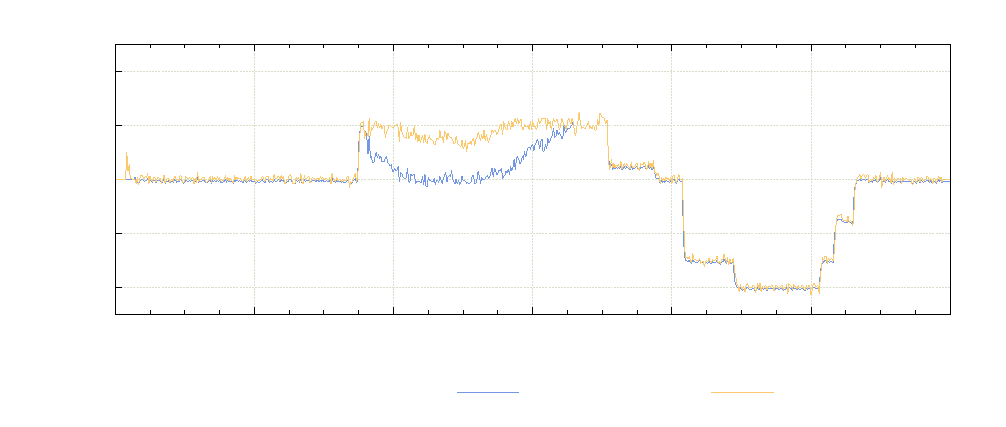
\includegraphics{Graphs/4/KUSResults/RefugePressure/RefugePressure}}%
    \gplfronttext
  \end{picture}%
\endgroup
}
		\caption{The Baseline system pressure compared to the system pressure when refuge bay leaks are reduce.}
		\label{fig: RefugeBay Pressures.}
	\end{figure}  
	Tested scenario where all excessive leaking valves are removed.
	Refuge bays savings 1MW E.E.
	
	\subsection{Scenario 2. Closing off levels/stopes}
	The effect of in-stope control during peak times was simulated for level 105L. The level was modelled to include all major leaks, refuge bays and drilling sections that were manually identified from the level investigations. This is shown in the simulation diagram shown in Figure For comparison, station isolation and the combination of in-stope control and station isolation were simulated. 
	
	\begin{figure}[h!]
		\centering
		\fbox{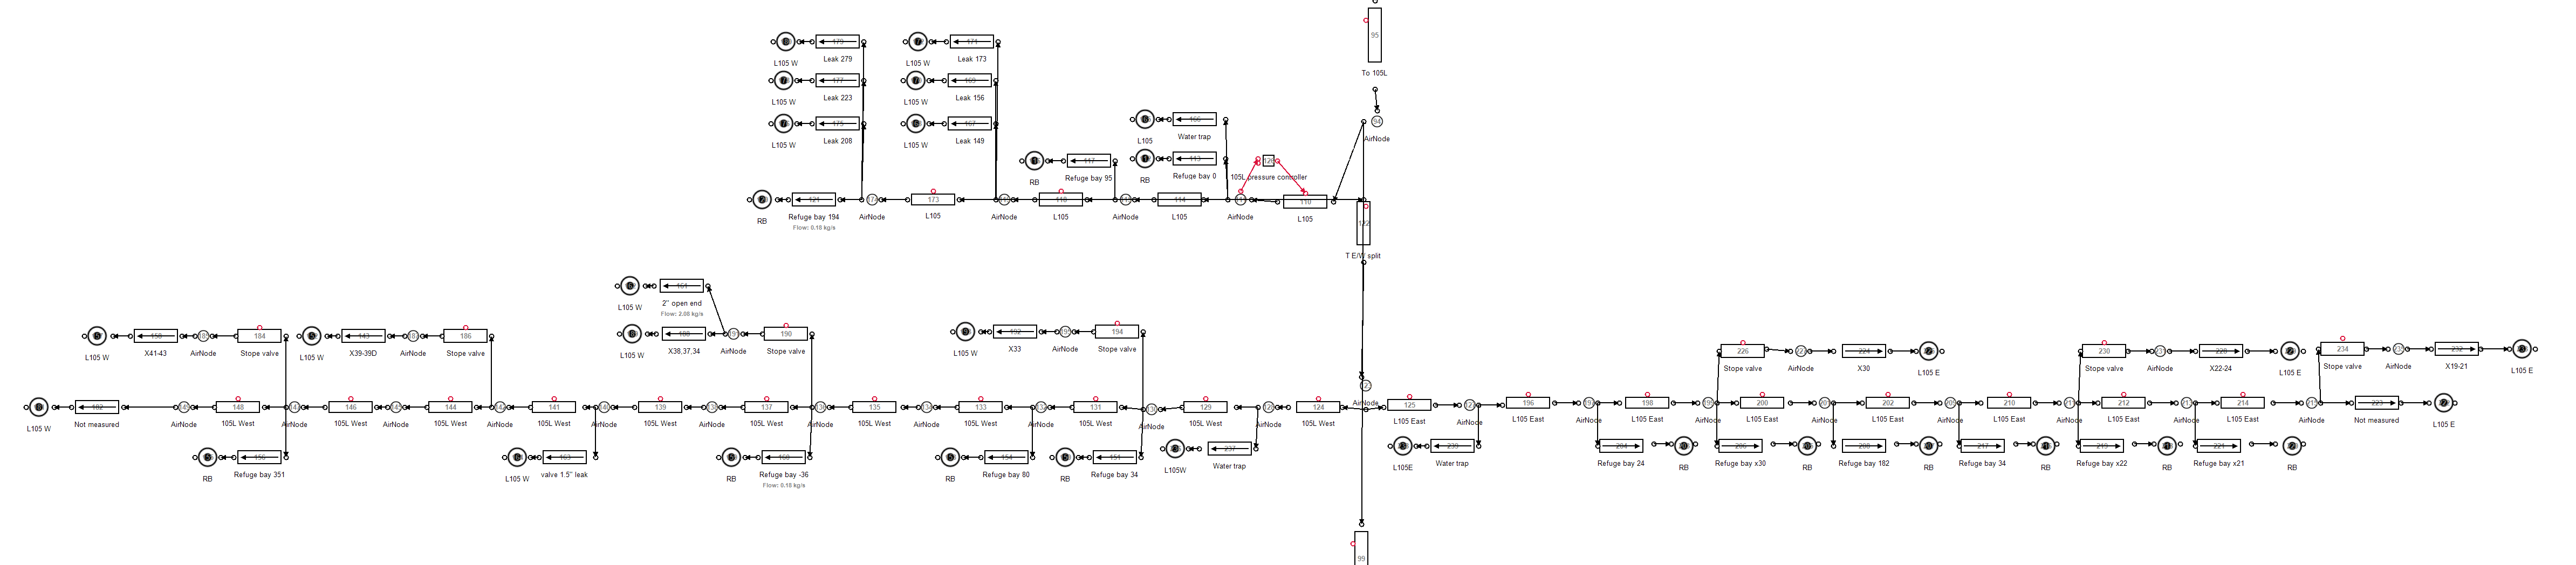
\includegraphics[width=\textwidth]{Images/4/StopeSim}}
		\caption{Underground level layout.}
		\label{fig: KUS Simulation level layout}
	\end{figure}	
	
	
	\subsection{Validation of results}
	
	- awaiting results on manual tests
	
	\subsection{Summary}
\newpage
\section{Periodic simulation analysis}
	\subsection{Preamble}
	Updating the inputs of a simulation periodically could be used to verify simulation model accuracy. If the precision of simulation outputs remains for subsequent days, this would indicate that the model is correctly calibrated. Additionally, this process could be used to identify significant operational changes that occur within the system. This would cause the simulation outputs to differ from the actual measured parameters. 
	\par 
	A Periodic simulation the method shown in Figure \ref{fig: PeriodicProcess} was developed for this analysis. Simulation input data is collected periodically for each simulation interval, this data includes only inputs that vary day to day such as schedules, air conditions and  measured flows. Once the input values are collected, they are then imported into the compressed air model. The simulation performed and the output data is exported for analysis. The  simulated data is then compared with the actual operation of the system and major discrepancies are identified. This process is repeated periodically.
		\begin{figure}[h]
		\centering
		\fbox{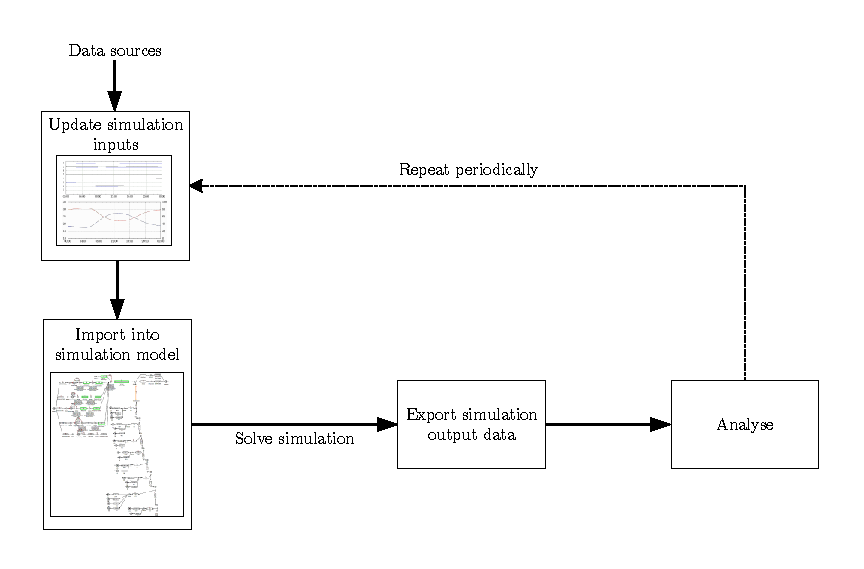
\includegraphics[trim =0cm 0.5cm 0cm 1cm,width=\textwidth]{Graphs/4/PeriodicProcess/PeriodicProcess.pdf}}
		\caption{The periodic simulation process that was followed in this analysis.}
		\label{fig: PeriodicProcess}
		\end{figure}	
	     \subsection{Results}
	     Daily periodic simulation was implemented between 2016/11/01 and 2016/11/30. For each period, the simulated total flow, shaft delivery pressure and total power consumption were compared to the actual operation. The results of this analysis are shown in Figure \ref{fig: Periodic simulation}.
	     \par 
	     
	\begin{figure}[h]
		\centering
		\fbox{% GNUPLOT: LaTeX picture with Postscript
\begingroup
  \makeatletter
  \providecommand\color[2][]{%
    \GenericError{(gnuplot) \space\space\space\@spaces}{%
      Package color not loaded in conjunction with
      terminal option `colourtext'%
    }{See the gnuplot documentation for explanation.%
    }{Either use 'blacktext' in gnuplot or load the package
      color.sty in LaTeX.}%
    \renewcommand\color[2][]{}%
  }%
  \providecommand\includegraphics[2][]{%
    \GenericError{(gnuplot) \space\space\space\@spaces}{%
      Package graphicx or graphics not loaded%
    }{See the gnuplot documentation for explanation.%
    }{The gnuplot epslatex terminal needs graphicx.sty or graphics.sty.}%
    \renewcommand\includegraphics[2][]{}%
  }%
  \providecommand\rotatebox[2]{#2}%
  \@ifundefined{ifGPcolor}{%
    \newif\ifGPcolor
    \GPcolortrue
  }{}%
  \@ifundefined{ifGPblacktext}{%
    \newif\ifGPblacktext
    \GPblacktextfalse
  }{}%
  % define a \g@addto@macro without @ in the name:
  \let\gplgaddtomacro\g@addto@macro
  % define empty templates for all commands taking text:
  \gdef\gplbacktext{}%
  \gdef\gplfronttext{}%
  \makeatother
  \ifGPblacktext
    % no textcolor at all
    \def\colorrgb#1{}%
    \def\colorgray#1{}%
  \else
    % gray or color?
    \ifGPcolor
      \def\colorrgb#1{\color[rgb]{#1}}%
      \def\colorgray#1{\color[gray]{#1}}%
      \expandafter\def\csname LTw\endcsname{\color{white}}%
      \expandafter\def\csname LTb\endcsname{\color{black}}%
      \expandafter\def\csname LTa\endcsname{\color{black}}%
      \expandafter\def\csname LT0\endcsname{\color[rgb]{1,0,0}}%
      \expandafter\def\csname LT1\endcsname{\color[rgb]{0,1,0}}%
      \expandafter\def\csname LT2\endcsname{\color[rgb]{0,0,1}}%
      \expandafter\def\csname LT3\endcsname{\color[rgb]{1,0,1}}%
      \expandafter\def\csname LT4\endcsname{\color[rgb]{0,1,1}}%
      \expandafter\def\csname LT5\endcsname{\color[rgb]{1,1,0}}%
      \expandafter\def\csname LT6\endcsname{\color[rgb]{0,0,0}}%
      \expandafter\def\csname LT7\endcsname{\color[rgb]{1,0.3,0}}%
      \expandafter\def\csname LT8\endcsname{\color[rgb]{0.5,0.5,0.5}}%
    \else
      % gray
      \def\colorrgb#1{\color{black}}%
      \def\colorgray#1{\color[gray]{#1}}%
      \expandafter\def\csname LTw\endcsname{\color{white}}%
      \expandafter\def\csname LTb\endcsname{\color{black}}%
      \expandafter\def\csname LTa\endcsname{\color{black}}%
      \expandafter\def\csname LT0\endcsname{\color{black}}%
      \expandafter\def\csname LT1\endcsname{\color{black}}%
      \expandafter\def\csname LT2\endcsname{\color{black}}%
      \expandafter\def\csname LT3\endcsname{\color{black}}%
      \expandafter\def\csname LT4\endcsname{\color{black}}%
      \expandafter\def\csname LT5\endcsname{\color{black}}%
      \expandafter\def\csname LT6\endcsname{\color{black}}%
      \expandafter\def\csname LT7\endcsname{\color{black}}%
      \expandafter\def\csname LT8\endcsname{\color{black}}%
    \fi
  \fi
    \setlength{\unitlength}{0.0500bp}%
    \ifx\gptboxheight\undefined%
      \newlength{\gptboxheight}%
      \newlength{\gptboxwidth}%
      \newsavebox{\gptboxtext}%
    \fi%
    \setlength{\fboxrule}{0.5pt}%
    \setlength{\fboxsep}{1pt}%
\begin{picture}(9360.00,4032.00)%
    \gplgaddtomacro\gplbacktext{%
      \colorrgb{0.00,0.00,0.00}%
      \put(814,924){\makebox(0,0)[r]{\strut{}$80$}}%
      \colorrgb{0.00,0.00,0.00}%
      \put(814,1635){\makebox(0,0)[r]{\strut{}$85$}}%
      \colorrgb{0.00,0.00,0.00}%
      \put(814,2346){\makebox(0,0)[r]{\strut{}$90$}}%
      \colorrgb{0.00,0.00,0.00}%
      \put(814,3056){\makebox(0,0)[r]{\strut{}$95$}}%
      \colorrgb{0.00,0.00,0.00}%
      \put(814,3767){\makebox(0,0)[r]{\strut{}$100$}}%
      \colorrgb{0.00,0.00,0.00}%
      \put(946,704){\makebox(0,0){\strut{}2016/11/01}}%
      \colorrgb{0.00,0.00,0.00}%
      \put(2604,704){\makebox(0,0){\strut{}2016/11/07}}%
      \colorrgb{0.00,0.00,0.00}%
      \put(4263,704){\makebox(0,0){\strut{}2016/11/13}}%
      \colorrgb{0.00,0.00,0.00}%
      \put(5921,704){\makebox(0,0){\strut{}2016/11/19}}%
      \colorrgb{0.00,0.00,0.00}%
      \put(7580,704){\makebox(0,0){\strut{}2016/11/25}}%
    }%
    \gplgaddtomacro\gplfronttext{%
      \csname LTb\endcsname%
      \put(176,2345){\rotatebox{-270}{\makebox(0,0){\strut{}Accuracy (\%)}}}%
      \put(4954,374){\makebox(0,0){\strut{}Date of simulation}}%
      \csname LTb\endcsname%
      \put(3143,173){\makebox(0,0)[r]{\strut{}Flow}}%
      \csname LTb\endcsname%
      \put(5054,173){\makebox(0,0)[r]{\strut{}Pressure}}%
      \csname LTb\endcsname%
      \put(6965,173){\makebox(0,0)[r]{\strut{}Power}}%
    }%
    \gplbacktext
    \put(0,0){\fbox{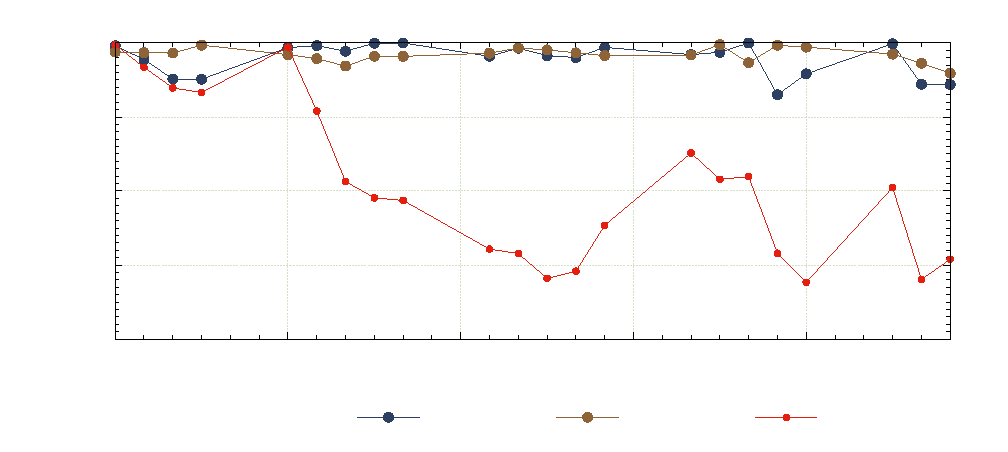
\includegraphics[trim=0 0 0.1cm 0, clip]{Graphs/4/Periodic1/Periodic1}}}%
    \gplfronttext
  \end{picture}%
\endgroup
}
		\caption{The flow, pressure and power error percentages for daily periodic simulations over a month.}
		\label{fig: Periodic simulation}
	\end{figure}   
The accuracy of the flow and pressure parameters of the model remained precise for the duration of the periodic simulation. However From the 2016/11/07, the accuracy of the simulated power dropped by between 10 and 15 percent. The daily average power of the system up to the point was approximately 12.5 MW, a 15\% simulation error therefore relates to 1.9 MW. This suggests a major shift in operation of the system.
\par 
A deeper analysis was performed to try ascertain the source of the operational change. From the analysis it was identified that the simulated power for compressor 1 no longer reflected the actual power measurement from the system. A look at the actual power measurement for compressor 1 showed a sharp decline in power starting from the 2016/11/07. At the same time the efficiency, or amount of power required per kg/s of air, for the system increased significantly. This is shown in Figure \ref{fig: MeasurementAccuracy.} the average daily power for compressor 1, shown in blue, and the air mass flow per Watt, shown in yellow, shift dramatically from the same. 
	\begin{figure}[h]
		\centering
		\fbox{% GNUPLOT: LaTeX picture with Postscript
\begingroup
  \makeatletter
  \providecommand\color[2][]{%
    \GenericError{(gnuplot) \space\space\space\@spaces}{%
      Package color not loaded in conjunction with
      terminal option `colourtext'%
    }{See the gnuplot documentation for explanation.%
    }{Either use 'blacktext' in gnuplot or load the package
      color.sty in LaTeX.}%
    \renewcommand\color[2][]{}%
  }%
  \providecommand\includegraphics[2][]{%
    \GenericError{(gnuplot) \space\space\space\@spaces}{%
      Package graphicx or graphics not loaded%
    }{See the gnuplot documentation for explanation.%
    }{The gnuplot epslatex terminal needs graphicx.sty or graphics.sty.}%
    \renewcommand\includegraphics[2][]{}%
  }%
  \providecommand\rotatebox[2]{#2}%
  \@ifundefined{ifGPcolor}{%
    \newif\ifGPcolor
    \GPcolortrue
  }{}%
  \@ifundefined{ifGPblacktext}{%
    \newif\ifGPblacktext
    \GPblacktextfalse
  }{}%
  % define a \g@addto@macro without @ in the name:
  \let\gplgaddtomacro\g@addto@macro
  % define empty templates for all commands taking text:
  \gdef\gplbacktext{}%
  \gdef\gplfronttext{}%
  \makeatother
  \ifGPblacktext
    % no textcolor at all
    \def\colorrgb#1{}%
    \def\colorgray#1{}%
  \else
    % gray or color?
    \ifGPcolor
      \def\colorrgb#1{\color[rgb]{#1}}%
      \def\colorgray#1{\color[gray]{#1}}%
      \expandafter\def\csname LTw\endcsname{\color{white}}%
      \expandafter\def\csname LTb\endcsname{\color{black}}%
      \expandafter\def\csname LTa\endcsname{\color{black}}%
      \expandafter\def\csname LT0\endcsname{\color[rgb]{1,0,0}}%
      \expandafter\def\csname LT1\endcsname{\color[rgb]{0,1,0}}%
      \expandafter\def\csname LT2\endcsname{\color[rgb]{0,0,1}}%
      \expandafter\def\csname LT3\endcsname{\color[rgb]{1,0,1}}%
      \expandafter\def\csname LT4\endcsname{\color[rgb]{0,1,1}}%
      \expandafter\def\csname LT5\endcsname{\color[rgb]{1,1,0}}%
      \expandafter\def\csname LT6\endcsname{\color[rgb]{0,0,0}}%
      \expandafter\def\csname LT7\endcsname{\color[rgb]{1,0.3,0}}%
      \expandafter\def\csname LT8\endcsname{\color[rgb]{0.5,0.5,0.5}}%
    \else
      % gray
      \def\colorrgb#1{\color{black}}%
      \def\colorgray#1{\color[gray]{#1}}%
      \expandafter\def\csname LTw\endcsname{\color{white}}%
      \expandafter\def\csname LTb\endcsname{\color{black}}%
      \expandafter\def\csname LTa\endcsname{\color{black}}%
      \expandafter\def\csname LT0\endcsname{\color{black}}%
      \expandafter\def\csname LT1\endcsname{\color{black}}%
      \expandafter\def\csname LT2\endcsname{\color{black}}%
      \expandafter\def\csname LT3\endcsname{\color{black}}%
      \expandafter\def\csname LT4\endcsname{\color{black}}%
      \expandafter\def\csname LT5\endcsname{\color{black}}%
      \expandafter\def\csname LT6\endcsname{\color{black}}%
      \expandafter\def\csname LT7\endcsname{\color{black}}%
      \expandafter\def\csname LT8\endcsname{\color{black}}%
    \fi
  \fi
    \setlength{\unitlength}{0.0500bp}%
    \ifx\gptboxheight\undefined%
      \newlength{\gptboxheight}%
      \newlength{\gptboxwidth}%
      \newsavebox{\gptboxtext}%
    \fi%
    \setlength{\fboxrule}{0.5pt}%
    \setlength{\fboxsep}{1pt}%
\begin{picture}(9360.00,3528.00)%
    \gplgaddtomacro\gplbacktext{%
      \colorrgb{0.00,0.00,0.00}%
      \put(946,924){\makebox(0,0)[r]{\strut{}$1000$}}%
      \colorrgb{0.00,0.00,0.00}%
      \put(946,1314){\makebox(0,0)[r]{\strut{}$1500$}}%
      \colorrgb{0.00,0.00,0.00}%
      \put(946,1704){\makebox(0,0)[r]{\strut{}$2000$}}%
      \colorrgb{0.00,0.00,0.00}%
      \put(946,2094){\makebox(0,0)[r]{\strut{}$2500$}}%
      \colorrgb{0.00,0.00,0.00}%
      \put(946,2483){\makebox(0,0)[r]{\strut{}$3000$}}%
      \colorrgb{0.00,0.00,0.00}%
      \put(946,2873){\makebox(0,0)[r]{\strut{}$3500$}}%
      \colorrgb{0.00,0.00,0.00}%
      \put(946,3263){\makebox(0,0)[r]{\strut{}$4000$}}%
      \colorrgb{0.00,0.00,0.00}%
      \put(1078,704){\makebox(0,0){\strut{}2016/09/01}}%
      \colorrgb{0.00,0.00,0.00}%
      \put(3118,704){\makebox(0,0){\strut{}2016/10/01}}%
      \colorrgb{0.00,0.00,0.00}%
      \put(5226,704){\makebox(0,0){\strut{}2016/11/01}}%
      \colorrgb{0.00,0.00,0.00}%
      \put(5226,704){\makebox(0,0){\strut{}2016/11/01}}%
      \colorrgb{0.00,0.00,0.00}%
      \put(7266,704){\makebox(0,0){\strut{}2016/12/01}}%
      \colorrgb{0.00,0.00,0.00}%
      \put(8214,924){\makebox(0,0)[l]{\strut{}$2$}}%
      \colorrgb{0.00,0.00,0.00}%
      \put(8214,1314){\makebox(0,0)[l]{\strut{}$2.5$}}%
      \colorrgb{0.00,0.00,0.00}%
      \put(8214,1704){\makebox(0,0)[l]{\strut{}$3$}}%
      \colorrgb{0.00,0.00,0.00}%
      \put(8214,2094){\makebox(0,0)[l]{\strut{}$3.5$}}%
      \colorrgb{0.00,0.00,0.00}%
      \put(8214,2483){\makebox(0,0)[l]{\strut{}$4$}}%
      \colorrgb{0.00,0.00,0.00}%
      \put(8214,2873){\makebox(0,0)[l]{\strut{}$4.5$}}%
      \colorrgb{0.00,0.00,0.00}%
      \put(8214,3263){\makebox(0,0)[l]{\strut{}$5$}}%
    }%
    \gplgaddtomacro\gplfronttext{%
      \csname LTb\endcsname%
      \put(176,2093){\rotatebox{-270}{\makebox(0,0){\strut{}Power (kW)}}}%
      \put(8851,2093){\rotatebox{-270}{\makebox(0,0){\strut{}$Flow per Watt (kg/s/W)$}}}%
      \put(4580,374){\makebox(0,0){\strut{}Date}}%
      \csname LTb\endcsname%
      \put(3725,173){\makebox(0,0)[r]{\strut{}Compressor 1 average power}}%
      \csname LTb\endcsname%
      \put(8012,173){\makebox(0,0)[r]{\strut{}System efficiency}}%
      \csname LTb\endcsname%
      \put(6220,3029){\makebox(0,0){\strut{}\shortstack{\small{Periodic simulation}}}}%
    }%
    \gplbacktext
    \put(0,0){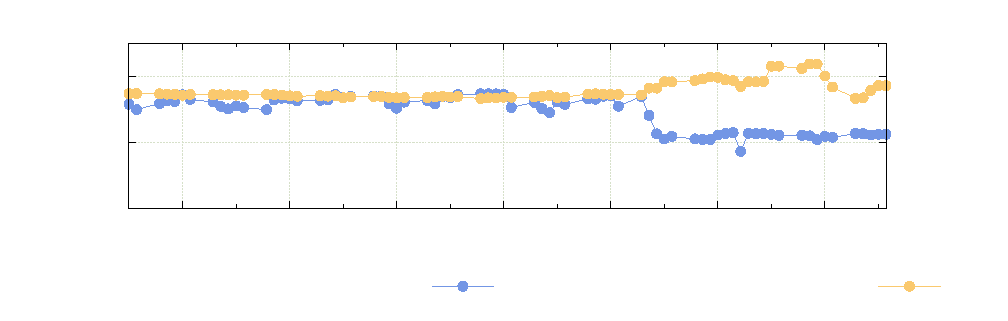
\includegraphics{Graphs/4/PeriodicRange/PeriodicRange}}%
    \gplfronttext
  \end{picture}%
\endgroup
}
		\caption{Supply efficiency and Compressor 1's average power output over the time of the periodic analysis.}
		\label{fig: MeasurementAccuracy.}
	\end{figure} 
   The results seem to show that there was a major change in the operation compressor 1 that effected the efficiency of the system. A more likely explanation is that there is a malfunction with the power meter. This explains the apparent increase in efficiency over the same period as a lower power is measure then is actually being utilised. In this scenario the simulated power measurement can retrospectively be used as a more accurate metric for the energy consumption of the system.  
   \subsection{Validation}
   To validate that the change identified using periodic simulation was caused by the power meter, data from the substation was compared to the combined individual compressors meters. This comparison is shown in Figure \ref{fig: Corrected Periodic simulation}. The comparison shows that the substation power measurement strays from the compressors at the same time that compressor 1 average daily power drops.
	\begin{figure}[h]
		\centering
		\fbox{% GNUPLOT: LaTeX picture with Postscript
\begingroup
  \makeatletter
  \providecommand\color[2][]{%
    \GenericError{(gnuplot) \space\space\space\@spaces}{%
      Package color not loaded in conjunction with
      terminal option `colourtext'%
    }{See the gnuplot documentation for explanation.%
    }{Either use 'blacktext' in gnuplot or load the package
      color.sty in LaTeX.}%
    \renewcommand\color[2][]{}%
  }%
  \providecommand\includegraphics[2][]{%
    \GenericError{(gnuplot) \space\space\space\@spaces}{%
      Package graphicx or graphics not loaded%
    }{See the gnuplot documentation for explanation.%
    }{The gnuplot epslatex terminal needs graphicx.sty or graphics.sty.}%
    \renewcommand\includegraphics[2][]{}%
  }%
  \providecommand\rotatebox[2]{#2}%
  \@ifundefined{ifGPcolor}{%
    \newif\ifGPcolor
    \GPcolortrue
  }{}%
  \@ifundefined{ifGPblacktext}{%
    \newif\ifGPblacktext
    \GPblacktextfalse
  }{}%
  % define a \g@addto@macro without @ in the name:
  \let\gplgaddtomacro\g@addto@macro
  % define empty templates for all commands taking text:
  \gdef\gplbacktext{}%
  \gdef\gplfronttext{}%
  \makeatother
  \ifGPblacktext
    % no textcolor at all
    \def\colorrgb#1{}%
    \def\colorgray#1{}%
  \else
    % gray or color?
    \ifGPcolor
      \def\colorrgb#1{\color[rgb]{#1}}%
      \def\colorgray#1{\color[gray]{#1}}%
      \expandafter\def\csname LTw\endcsname{\color{white}}%
      \expandafter\def\csname LTb\endcsname{\color{black}}%
      \expandafter\def\csname LTa\endcsname{\color{black}}%
      \expandafter\def\csname LT0\endcsname{\color[rgb]{1,0,0}}%
      \expandafter\def\csname LT1\endcsname{\color[rgb]{0,1,0}}%
      \expandafter\def\csname LT2\endcsname{\color[rgb]{0,0,1}}%
      \expandafter\def\csname LT3\endcsname{\color[rgb]{1,0,1}}%
      \expandafter\def\csname LT4\endcsname{\color[rgb]{0,1,1}}%
      \expandafter\def\csname LT5\endcsname{\color[rgb]{1,1,0}}%
      \expandafter\def\csname LT6\endcsname{\color[rgb]{0,0,0}}%
      \expandafter\def\csname LT7\endcsname{\color[rgb]{1,0.3,0}}%
      \expandafter\def\csname LT8\endcsname{\color[rgb]{0.5,0.5,0.5}}%
    \else
      % gray
      \def\colorrgb#1{\color{black}}%
      \def\colorgray#1{\color[gray]{#1}}%
      \expandafter\def\csname LTw\endcsname{\color{white}}%
      \expandafter\def\csname LTb\endcsname{\color{black}}%
      \expandafter\def\csname LTa\endcsname{\color{black}}%
      \expandafter\def\csname LT0\endcsname{\color{black}}%
      \expandafter\def\csname LT1\endcsname{\color{black}}%
      \expandafter\def\csname LT2\endcsname{\color{black}}%
      \expandafter\def\csname LT3\endcsname{\color{black}}%
      \expandafter\def\csname LT4\endcsname{\color{black}}%
      \expandafter\def\csname LT5\endcsname{\color{black}}%
      \expandafter\def\csname LT6\endcsname{\color{black}}%
      \expandafter\def\csname LT7\endcsname{\color{black}}%
      \expandafter\def\csname LT8\endcsname{\color{black}}%
    \fi
  \fi
    \setlength{\unitlength}{0.0500bp}%
    \ifx\gptboxheight\undefined%
      \newlength{\gptboxheight}%
      \newlength{\gptboxwidth}%
      \newsavebox{\gptboxtext}%
    \fi%
    \setlength{\fboxrule}{0.5pt}%
    \setlength{\fboxsep}{1pt}%
\begin{picture}(9360.00,4284.00)%
    \gplgaddtomacro\gplbacktext{%
      \colorrgb{0.00,0.00,0.00}%
      \put(682,1366){\makebox(0,0)[r]{\strut{}$8$}}%
      \colorrgb{0.00,0.00,0.00}%
      \put(682,2250){\makebox(0,0)[r]{\strut{}$10$}}%
      \colorrgb{0.00,0.00,0.00}%
      \put(682,3135){\makebox(0,0)[r]{\strut{}$12$}}%
      \colorrgb{0.00,0.00,0.00}%
      \put(682,4019){\makebox(0,0)[r]{\strut{}$14$}}%
      \colorrgb{0.00,0.00,0.00}%
      \put(1938,704){\makebox(0,0){\strut{}05/11/2016}}%
      \colorrgb{0.00,0.00,0.00}%
      \put(3343,704){\makebox(0,0){\strut{}10/11/2016}}%
      \colorrgb{0.00,0.00,0.00}%
      \put(4748,704){\makebox(0,0){\strut{}15/11/2016}}%
      \colorrgb{0.00,0.00,0.00}%
      \put(6152,704){\makebox(0,0){\strut{}20/11/2016}}%
      \colorrgb{0.00,0.00,0.00}%
      \put(7557,704){\makebox(0,0){\strut{}25/11/2016}}%
      \colorrgb{0.00,0.00,0.00}%
      \put(8962,704){\makebox(0,0){\strut{}30/11/2016}}%
    }%
    \gplgaddtomacro\gplfronttext{%
      \csname LTb\endcsname%
      \put(176,2471){\rotatebox{-270}{\makebox(0,0){\strut{}Power (MW)}}}%
      \put(4888,374){\makebox(0,0){\strut{}Date}}%
      \csname LTb\endcsname%
      \put(4033,173){\makebox(0,0)[r]{\strut{}Compressor power measrement}}%
      \csname LTb\endcsname%
      \put(8452,173){\makebox(0,0)[r]{\strut{}Independant measurement}}%
    }%
    \gplbacktext
    \put(0,0){\fbox{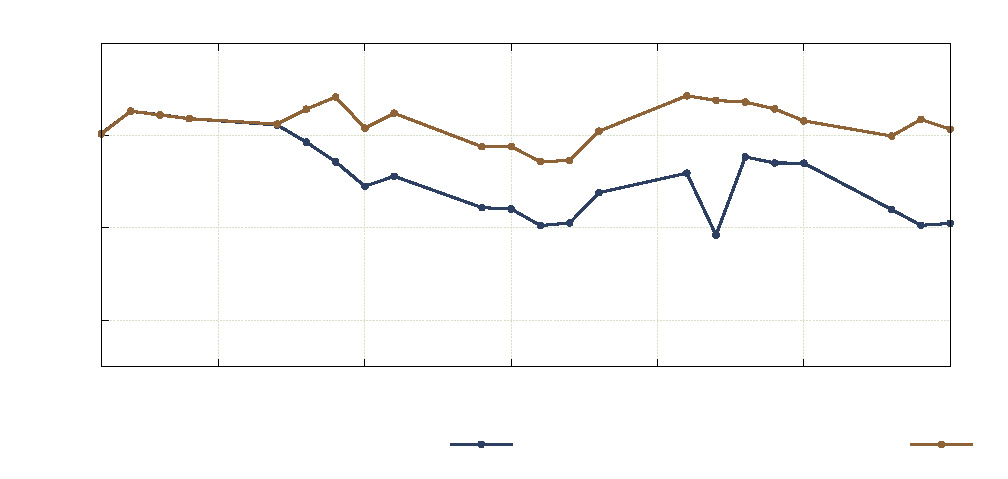
\includegraphics[trim=0 0 0.1cm 0, clip]{Graphs/4/PeriodicValidation/PeriodicValidation}}}%
    \gplfronttext
  \end{picture}%
\endgroup
}
		\caption{Comparison using alternative power source.}
		\label{fig: Corrected Periodic simulation}
	\end{figure}    
	
	\subsection{Summary}
\newpage
\section{Potential benefit for SA mines}

	Using  
\section{Conclusion}